%% abtex2-modelo-trabalho-academico.tex, v-1.9.7 laurocesar
%% Copyright 2012-2018 by abnTeX2 group at http://www.abntex.net.br/ 
%%
%% This work may be distributed and/or modified under the
%% conditions of the LaTeX Project Public License, either version 1.3
%% of this license or (at your option) any later version.
%% The latest version of this license is in
%%   http://www.latex-project.org/lppl.txt
%% and version 1.3 or later is part of all distributions of LaTeX
%% version 2005/12/01 or later.
%%
%% This work has the LPPL maintenance status `maintained'.
%% 
%% The Current Maintainer of this work is the abnTeX2 team, led
%% by Lauro César Araujo. Further information are available on 
%% http://www.abntex.net.br/
%%
%% This work consists of the files abntex2-modelo-trabalho-academico.tex,
%% abntex2-modelo-include-comandos and abntex2-modelo-references.bib
%%
% ------------------------------------------------------------------------
% ------------------------------------------------------------------------
% abnTeX2: Modelo de Trabalho Academico (tese de doutorado, dissertacao de
% mestrado e trabalhos monograficos em geral) em conformidade com 
% ABNT NBR 14724:2011: Informacao e documentacao - Trabalhos academicos -
% Apresentacao
% ------------------------------------------------------------------------
% ------------------------------------------------------------------------
%%
%% Documento ajustado para PCS-EPUSP em 15/mar/2023 por Cintia Borges Margi
% ------------------------------------------------------------------------
%%
\documentclass[
	% -- opções da classe memoir --
	12pt,				% tamanho da fonte
	openright,			% capítulos começam em pág ímpar (insere página vazia caso preciso)
	twoside,			% para impressão em recto e verso. Oposto a oneside
	a4paper,			% tamanho do papel. 
	% -- opções da classe abntex2 --
	%chapter=TITLE,		% títulos de capítulos convertidos em letras maiúsculas
	%section=TITLE,		% títulos de seções convertidos em letras maiúsculas
	%subsection=TITLE,	% títulos de subseções convertidos em letras maiúsculas
	%subsubsection=TITLE,% títulos de subsubseções convertidos em letras maiúsculas
	% -- opções do pacote babel --
  sumario=tradicional,
	english,			% idioma adicional para hifenização
	french,				% idioma adicional para hifenização
	spanish,			% idioma adicional para hifenização
	brazil				% o último idioma é o principal do documento
	]{abntex2}

% ---
% Pacotes básicos 
% ---
% \usepackage{lmodern}			% Usa a fonte Latin Modern
% \usepackage[mono=false]{libertinus}
% \usepackage[scale=1]{libertinust1math}
% \usepackage{librecaslon}
% \usepackage{tgpagella}
\usepackage{mathpazo}
\usepackage[scale=0.9]{sourcecodepro}
\usepackage[T1]{fontenc}		% Selecao de codigos de fonte.
\usepackage[utf8]{inputenc}		% Codificacao do documento (conversão automática dos acentos)
\usepackage{indentfirst}		% Indenta o primeiro parágrafo de cada seção.
\usepackage{color}				% Controle das cores
\usepackage{graphicx}			% Inclusão de gráficos
\usepackage{microtype} 			% para melhorias de justificação
\usepackage{lipsum}
\usepackage[brazilian,hyperpageref]{backref}	 % Paginas com as citações na bibl
\usepackage[alf]{abntex2cite}	% Citações padrão ABNT
\usepackage[final]{pdfpages}
\usepackage{amsmath}
\usepackage{siunitx}
\usepackage{gensymb}
\usepackage{textcomp}
\usepackage{amssymb}
\usepackage{amsfonts}
\usepackage[hyperref,svgnames,x11names,table,dvipsnames]{xcolor}
\usepackage{scrbase}
\usepackage{listings}
\usepackage[percent]{overpic}
\usepackage{tikz}
\usepackage{smartdiagram}
\usepackage{multirow}
\usepackage{afterpage}
\usesmartdiagramlibrary{additions}
\newcaptionname{brazil}{\lstlistingname}{Listagem}

\definecolor{codegreen}{rgb}{0,0.6,0}
\definecolor{codegray}{rgb}{0.5,0.5,0.5}
\definecolor{codepurple}{rgb}{0.5,0.1,0.82}
\definecolor{codeblue}{rgb}{0.1,0.1,0.86}
\lstdefinestyle{mystyle}{
    commentstyle=\color{codegreen},
    keywordstyle=\color{codeblue},
    numberstyle=\ttfamily\color{codegray},
    stringstyle=\color{BrickRed},
    basicstyle=\ttfamily,
    breakatwhitespace=false,         
    breaklines=true,                 
    captionpos=t,                    
    keepspaces=true,
    numbers=left,
    numbersep=5pt,
    showspaces=false,
    showstringspaces=false,
    showtabs=false,
    tabsize=2,
    frame=single,
}
\lstset{style=mystyle}

% \smartdiagramset{back arrow disabled=true,
  %   text width=.3\textwidth,
  %   uniform color list=white for all items,
  %   uniform arrow color=true,
  %   arrow color=black!70,
  %   border color=black!70,
  %   arrow line width=2pt,
  %   additions={additional arrow color=black!70,
  %       additional arrow line width=2pt}}
  % \tikzset{every shadow/.style={fill=none,shadow scale=0},
  %   module/.append style={very thick}}
  % {\color{lightgray}\framebox[.6\textwidth]{
  %     \smartdiagramadd[flow diagram]{%
  %       General framework (Section \ref{sec:magnitude}),
  %       Literature study,
  %       Data-analysis,
  %       Model set-up\\ (SB \& NH),
  %       Simulations,
  %       Sensitivity analysis,
  %       Model update,
  %       Conclusions and recommendations}{}
  %     \begin{tikzpicture}[remember picture, overlay]
  %       \draw[additional item arrow type] (module7) -- ([xshift=25pt]module7.east) |- (module6);
  %       \draw[additional item arrow type] (module7) -- ([xshift=-25pt]module7.west) |- (module5);
  %     \end{tikzpicture}}}
\newcommand{\simpleflowdiagram}[2]{%
  \begin{center}
  \smartdiagramset{%
    back arrow disabled=true,
    text width=#1\textwidth,
    uniform color list=white for all items,
    uniform arrow color=true,
    arrow color=black!70,
    border color=black!70,
    arrow line width=2pt,
    additions={%
      additional arrow color=black!70,
      additional arrow line width=2pt%
    }%
  }
  \tikzset{%
    every shadow/.style={fill=none,shadow scale=0},
    module/.append style={very thick}%
  }
  \smartdiagramadd[flow diagram]{#2}{}%
  \end{center}
}



\newcommand{\chaptersep}{~}


% --- 
% CONFIGURAÇÕES DE PACOTES
% --- 
\DeclareSIUnit\angstrom{\text {Å}}
\newcommand{\citealp}[1]{\citeauthor{#1}, \citeyear{#1}}

% ---
% Configurações do pacote backref
% Usado sem a opção hyperpageref de backref
\renewcommand{\backrefpagesname}{Citado na(s) página(s):~}
% Texto padrão antes do número das páginas
\renewcommand{\backref}{}
% Define os textos da citação
\renewcommand*{\backrefalt}[4]{
	\ifcase #1 %
		Nenhuma citação no texto.%
	\or
		Citado na página #2.%
	\else
		Citado #1 vezes nas páginas #2.%
	\fi}%
% ---

% ---
% Informações de dados para CAPA e FOLHA DE ROSTO
% ---
\titulo{Sistema Inteligente para Busca de Objetos Astronômicos por Similaridade Visual usando Aprendizagem Profunda}
\autor{Natanael Magalhães Cardoso}
\local{São Paulo, SP}
\data{2024}
\orientador{Prof. Dr. António Mauro Saraiva}
\coorientador{Profa. Dra. Cláudia Mendes de Oliveira}
\instituicao{%
  Universidade de São Paulo -- USP
  \par
  Escola Politécnica
  \par
  Departamento de Engenharia de Computação e Sistemas Digitais (PCS)}
\tipotrabalho{Monografia de Conclusão de curso (Graduação)}
% O preambulo deve conter o tipo do trabalho, o objetivo, 
% o nome da instituição e a área de concentração 
\preambulo{Trabalho de conclusão de curso apresentado ao Departamento de Engenharia de Computação e Sistemas Digitais da Escola Politécnica da Universidade de São Paulo para obtenção do Título de Engenheiro.}
% ---


% ---
% Configurações de aparência do PDF final

% alterando o aspecto da cor azul
% \definecolor{blue}{RGB}{41,5,195}
\definecolor{blue}{HTML}{1A3280}

% informações do PDF
\makeatletter
\hypersetup{
     	%pagebackref=true,
		pdftitle={\@title}, 
		pdfauthor={\@author},
    	pdfsubject={\imprimirpreambulo},
	    pdfcreator={LaTeX with abnTeX2},
		pdfkeywords={abnt}{latex}{abntex}{abntex2}{trabalho acadêmico}, 
		colorlinks=true,       		% false: boxed links; true: colored links
    	linkcolor=BrickRed!92!black,          	% color of internal links
    	citecolor=BrickRed!92!black,        		% color of links to bibliography
		  urlcolor=BrickRed!92!black,
    	filecolor=magenta,      		% color of file links
      allbordercolors=white,
		bookmarksdepth=4
}
\makeatother
% --- 

% ---
% Posiciona figuras e tabelas no topo da página quando adicionadas sozinhas
% em um página em branco. Ver https://github.com/abntex/abntex2/issues/170
\makeatletter
\setlength{\@fptop}{5pt} % Set distance from top of page to first float
\makeatother
% ---

% ---
% Possibilita criação de Quadros e Lista de quadros.
% Ver https://github.com/abntex/abntex2/issues/176
%
\newcommand{\quadroname}{Quadro}
\newcommand{\listofquadrosname}{Lista de quadros}

\newfloat[chapter]{quadro}{loq}{\quadroname}
\newlistof{listofquadros}{loq}{\listofquadrosname}
\newlistentry{quadro}{loq}{0}

% configurações para atender às regras da ABNT
\setfloatadjustment{quadro}{\centering}
\counterwithout{quadro}{chapter}
\renewcommand{\cftquadroname}{\quadroname\space} 
\renewcommand*{\cftquadroaftersnum}{\hfill--\hfill}

\setfloatlocations{quadro}{hbtp} % Ver https://github.com/abntex/abntex2/issues/176
% ---

% --- 
% Espaçamentos entre linhas e parágrafos 
% --- 

% O tamanho do parágrafo é dado por:
\setlength{\parindent}{1.3cm}

% Controle do espaçamento entre um parágrafo e outro:
\setlength{\parskip}{0.2cm}  % tente também \onelineskip

% ---
% compila o indice
% ---
\makeindex
% ---










% ----
% Início do documento
% ----
\begin{document}
% Seleciona o idioma do documento (conforme pacotes do babel)
%\selectlanguage{english}
\selectlanguage{brazil}

% Retira espaço extra obsoleto entre as frases.
\frenchspacing

% ----------------------------------------------------------
% ELEMENTOS PRÉ-TEXTUAIS
% ----------------------------------------------------------
% \pretextual

% ---
% Capa
% ---
\imprimircapa
% ---

% ---
% Folha de rosto
% (o * indica que haverá a ficha bibliográfica)
% ---
\imprimirfolhaderosto*
% ---

% ---
% Inserir a ficha bibliografica
% ---

% Isto é um exemplo de Ficha Catalográfica, ou ``Dados internacionais de
% catalogação-na-publicação''. Você pode utilizar este modelo como referência. 
% Porém, provavelmente a biblioteca da sua universidade lhe fornecerá um PDF
% com a ficha catalográfica definitiva após a defesa do trabalho. Quando estiver
% com o documento, salve-o como PDF no diretório do seu projeto e substitua todo
% o conteúdo de implementação deste arquivo pelo comando abaixo:
%
%% TODO: utilizar a ficha catalográfica gerada em https://www.poli.usp.br/bibliotecas/servicos/catalogacao-na-publicacao
\begin{fichacatalografica}
  \includepdf{ficha_catalografica.pdf}
\end{fichacatalografica}

% \begin{fichacatalografica}
% 	\sffamily
% 	\vspace*{\fill}					% Posição vertical
% 	\begin{center}					% Minipage Centralizado
% 	\fbox{\begin{minipage}[c][8cm]{13.5cm}		% Largura
% 	\small
% 	\imprimirautor
% 	%Sobrenome, Nome do autor

% 	\hspace{0.5cm} \imprimirtitulo  / \imprimirautor. --
% 	\imprimirlocal, \imprimirdata-

% 	\hspace{0.5cm} \thelastpage p. : il. (algumas color.) ; 30 cm.\\

% 	\hspace{0.5cm} \imprimirorientadorRotulo~\imprimirorientador\\

% 	\hspace{0.5cm}
% 	\parbox[t]{\textwidth}{\imprimirtipotrabalho~--~\imprimirinstituicao,
% 	\imprimirdata.}\\

% 	\hspace{0.5cm}
% 		1. Palavra-chave1.
% 		2. Palavra-chave2.
% 		3. Palavra-chave3.
% 		I. Orientador.
% 		II. Universidade xxx.
% 		III. Faculdade de xxx.
% 		IV. Título 			
% 	\end{minipage}}
% 	\end{center}
% \end{fichacatalografica}
% ---

% ---
% Inserir errata
% ---
% \begin{errata}
% Elemento opcional da \citeonline[4.2.1.2]{NBR14724:2011}. Exemplo:

% \vspace{\onelineskip}

% FERRIGNO, C. R. A. \textbf{Tratamento de neoplasias ósseas apendiculares com
% reimplantação de enxerto ósseo autólogo autoclavado associado ao plasma
% rico em plaquetas}: estudo crítico na cirurgia de preservação de membro em
% cães. 2011. 128 f. Tese (Livre-Docência) - Faculdade de Medicina Veterinária e
% Zootecnia, Universidade de São Paulo, São Paulo, 2011.

% \begin{table}[htb]
% \center
% \footnotesize
% \begin{tabular}{|p{1.4cm}|p{1cm}|p{3cm}|p{3cm}|}
%   \hline
%    \textbf{Folha} & \textbf{Linha}  & \textbf{Onde se lê}  & \textbf{Leia-se}  \\
%     \hline
%     1 & 10 & auto-conclavo & autoconclavo\\
%    \hline
% \end{tabular}
% \end{table}

% \end{errata}
% ---

% ---
% Inserir folha de aprovação
% ---

% Isto é um exemplo de Folha de aprovação, elemento obrigatório da NBR
% 14724/2011 (seção 4.2.1.3). Você pode utilizar este modelo até a aprovação
% do trabalho. Após isso, substitua todo o conteúdo deste arquivo por uma
% imagem da página assinada pela banca com o comando abaixo:
%
% \begin{folhadeaprovacao}
% \includepdf{folhadeaprovacao_final.pdf}
% \end{folhadeaprovacao}
%
% \begin{folhadeaprovacao}

%   \begin{center}
%     {\ABNTEXchapterfont\large\imprimirautor}

%     \vspace*{\fill}\vspace*{\fill}
%     \begin{center}
%       \ABNTEXchapterfont\bfseries\Large\imprimirtitulo
%     \end{center}
%     \vspace*{\fill}

%     \hspace{.45\textwidth}
%     \begin{minipage}{.5\textwidth}
%         \imprimirpreambulo
%     \end{minipage}%
%     \vspace*{\fill}
%    \end{center}

%    Trabalho aprovado. \imprimirlocal, 24 de novembro de 2012:

%    \assinatura{\textbf{\imprimirorientador} \\ Orientador} 
%    \assinatura{\textbf{Professor} \\ Convidado 1}
%    \assinatura{\textbf{Professor} \\ Convidado 2}
%    %\assinatura{\textbf{Professor} \\ Convidado 3}
%    %\assinatura{\textbf{Professor} \\ Convidado 4}

%    \begin{center}
%     \vspace*{0.5cm}
%     {\large\imprimirlocal}
%     \par
%     {\large\imprimirdata}
%     \vspace*{1cm}
%   \end{center}

% \end{folhadeaprovacao}
% ---

% ---
% Dedicatória
% ---
\begin{dedicatoria}
  \vspace*{\fill}
  \centering
  \noindent
  \textit{Este trabalho é dedicado às crianças adultas que,\\
    quando pequenas, sonharam em se tornar cientistas.} \vspace*{\fill}
\end{dedicatoria}
% ---

% ---
% Agradecimentos
% ---
\begin{agradecimentos}
  Este trabalho foi possível graças à participação de centenas de milhares de voluntários em seis campanhas no projeto de ciência cidadã Galaxy Zoo.

  % As sugestões e diálogos com a Profa. Dra. Claudia Mendes de Oliveira do Departamento de Astronomia do IAG-USP foram fundamentais para o desenvolvimento deste projeto.

  Os modelos de aprendizagem profunda foram treinados utilizando recursos computacionais do Centro Brasileiro de Pesquisas Físicas (CBPF) e do Instituto de Astronomia, Geofísica e Ciências Atmosféricas da Universidade de São Paulo (IAG-USP).

  Os Legacy Surveys consistem em três projetos individuais e complementares: o Dark Energy Camera Legacy Survey (DECaLS; ID da proposta n$^o$ 2014B-0404; PIs: David Schlegel e Arjun Dey), o Beijing-Arizona Sky Survey (BASS; ID da prop. NOAO n$^o$ 2015A-0801; PIs: Zhou Xu e Xiaohui Fan) e o Mayall z-band Legacy Survey (MzLS; ID da prop. n$^o$ 2016A-0453; PI: Arjun Dey). DECaLS, BASS e MzLS juntos incluem dados obtidos, respectivamente, no telescópio Blanco, Observatório Interamericano Cerro Tololo, NOIRLab da NSF; o telescópio Bok, Observatório Steward, Universidade do Arizona; e o telescópio Mayall, Observatório Nacional Kitt Peak, NOIRLab. O processamento do pipeline e as análises dos dados foram apoiados pelo NOIRLab e pelo Laboratório Nacional Lawrence Berkeley (LBNL).

  Este projeto foi financiado com uma bolsa CAPES/CNPq.
\end{agradecimentos}
% ---

% ---
% Epígrafe
% ---
% \begin{epigrafe}
%     \vspace*{\fill}
% 	\begin{flushright}
% 		\textit{...}
% 	\end{flushright}
% \end{epigrafe}
% ---

% ---
% RESUMOS
% ---

% resumo em português
\setlength{\absparsep}{18pt} % ajusta o espaçamento dos parágrafos do resumo
\begin{resumo}
  Com o aumento exponencial na geração de dados astronômicos, impulsionado por levantamentos astronômicos modernos, a análise manual tornou-se inviável, demandando soluções computacionais eficientes. O objetivo principal foi criar uma ferramenta que automatizasse a identificação e a análise de objetos celestes com propriedades visuais semelhantes, promovendo avanços na pesquisa astronômica. O sistema proposto baseia-se em redes neurais convolucionais (CNNs) treinadas com imagens astronômicas, utilizando a transferência de aprendizado para otimizar a extração de representações visuais (também chamadas de \emph{embeddings}). Essas representações são vetores que codificam as características morfológicas e estruturais das galáxias, permitindo a busca e a recuperação de imagens semelhantes com alta precisão. A arquitetura do sistema inclui uma base de dados escalável para o armazenamento e indexação dos vetores de representação, além de uma interface web responsiva que facilita o uso por pesquisadores. Adicionalmente, o sistema incorpora técnicas de pré-processamento, como ajuste de campo de visão angular e aumento de dados, para garantir a qualidade e a representatividade dos conjuntos de treinamento. Os resultados obtidos evidenciam a eficácia do sistema em identificar padrões visuais entre galáxias, com avaliações robustas utilizando métricas como precisão média (mAP) e matrizes de confusão. Exemplos de buscas realizadas mostraram a aplicabilidade prática do sistema, que é capaz de entregar resultados relevantes mesmo em cenários desafiadores. Além disso, a interface gráfica desenvolvida provou-se intuitiva e eficiente, permitindo que usuários com diferentes níveis de expertise interajam com o sistema e explorem grandes volumes de dados de forma acessível. Por fim, o trabalho destaca também a importância da interdisciplinaridade entre ciência da computação e astronomia. A integração de técnicas de visão computacional, ciência de dados e práticas de engenharia de software resultou em uma solução que atende às demandas científicas e técnicas do domínio astronômico.

  \textbf{Palavras-chave}: aprendizagem profunda. visão computacional. astronomia.
\end{resumo}

% resumo em inglês
\begin{resumo}[Abstract]
  \begin{otherlanguage*}{english}
    With the exponential increase in astronomical data generation, driven by modern astronomical surveys, manual analysis has become unfeasible, demanding efficient computational solutions. The main objective was to create a tool that would automate the identification and analysis of celestial objects with similar visual properties, promoting advances in astronomical research. The proposed system is based on convolutional neural networks (CNNs) trained with astronomical images, using transfer learning to optimize the extraction of visual representations (also called embeddings). These representations are vectors that encode the morphological and structural characteristics of galaxies, allowing the search and retrieval of similar images with high precision. The system architecture includes a scalable database for storing and indexing representation vectors, as well as a responsive web interface that facilitates use by researchers. Additionally, the system incorporates preprocessing techniques, such as angular field of view adjustment and data augmentation, to ensure the quality and representativeness of the training sets. The results obtained demonstrate the effectiveness of the system in identifying visual patterns between galaxies, with robust evaluations using metrics such as mean precision (mAP) and confusion matrices. Examples of searches carried out showed the practical applicability of the system, which is capable of delivering relevant results even in challenging scenarios. In addition, the developed graphical interface proved to be intuitive and efficient, allowing users with different levels of expertise to interact with the system and explore large volumes of data in an accessible way. Finally, the work also highlights the importance of interdisciplinarity between computer science and astronomy. The integration of computer vision techniques, data science, and software engineering practices resulted in a solution that meets the scientific and technical demands of the astronomical domain.

    \vspace{\onelineskip}

    \noindent
    \textbf{Keywords}: deep learning. computer vision. astronomy.
  \end{otherlanguage*}
\end{resumo}

% % resumo em francês 
% \begin{resumo}[Résumé]
%  \begin{otherlanguage*}{french}
%     Il s'agit d'un résumé en français.

%    \textbf{Mots-clés}: latex. abntex. publication de textes.
%  \end{otherlanguage*}
% \end{resumo}

% % resumo em espanhol
% \begin{resumo}[Resumen]
%  \begin{otherlanguage*}{spanish}
%    Este es el resumen en español.

%    \textbf{Palabras clave}: latex. abntex. publicación de textos.
%  \end{otherlanguage*}
% \end{resumo}
% ---

% ---
% inserir lista de ilustrações
% ---
\pdfbookmark[0]{\listfigurename}{lof}
\listoffigures*
\cleardoublepage
% ---

% ---
% inserir lista de quadros
% ---
% \pdfbookmark[0]{\listofquadrosname}{loq}
% \listofquadros*
% \cleardoublepage
% ---

% ---
% inserir lista de tabelas
% ---
\pdfbookmark[0]{\listtablename}{lot}
\listoftables*
\cleardoublepage
% ---

% ---
% inserir lista de abreviaturas e siglas
% ---
\begin{siglas}
  \item[ADQL] Astronomical Data Query Language (Linguagem de Consulta de Dados Astronômicos)
  \item[API] Application Programming Interface (Interface de Programação de Aplicativos)
  \item[CBIR] Content-Based Image Retrieval (Recuperação de Imagem Baseada em Conteúdo)
  \item[CNN] Convolutional Neural Network (Rede Neural Convolucional)
  \item[CS] Citizen Science (Ciência Cidadã)
  \item[CV] Computer Vision (Visão Computacional)
  \item[Dec] Declination (Declinação, latitude)
  \item[DL] Deep Learning (Aprendizagem Profunda)
  \item[DR] Data Release (Liberação dos Dados)
  \item[FITS] Flexible Image Transport System (Sistema de Transporte de Imagem Flexível)
  \item[FLOPS] Floating-point Operations Per Second (Operações de Ponto flutuante Por Segundo)
  \item[FOV] Field of View (Campo de Visão)
  \item[GUI] Graphical User Interface (Interface Gráfica de Usuário)
  \item[IVOA] International Virtual Observatory Alliance (Aliança Internacional de Observatórios Virtuais)
  \item[LSST] Legacy Survey of Space and Time (Levantamento Legado do Espaço e do Tempo)
  \item[ML] Machine Learning (Aprendizagem de Máquina)
  \item[RA] Right Ascencion (Ascenção Reta, longitude)
  \item[SDSS] Sloan Digital Sky Survey
  \item[S-PLUS] Southern Photometric Local Universe Survey (Levantamento Fotométrico do Universo Local do Sul)
  \item[SQL] Structured Query Language (Linguagem de Consulta Estruturada)
  \item[VO] Virtual Observatory (Observatório Virtual)
\end{siglas}
% ---

% ---
% inserir lista de símbolos
% ---
\begin{simbolos}
  \item[$ \alpha $] Ascenção Reta (longitude)
  \item[$ \delta $] Declinação (latitude)
  \item[$R_e$] Raio efetivo da galáxia
  \item[$r_{\mathrm{mag}}$] Magnitude na banda r
\end{simbolos}
% ---

% ---
% inserir o sumario
% ---
\pdfbookmark[0]{\contentsname}{toc}
\tableofcontents*
\cleardoublepage
% ---


% ----------------------------------------------------------
% ELEMENTOS TEXTUAIS
% ----------------------------------------------------------
\textual


\section{Introdução}
\label{cap:introducao}

Com o avanço das tecnologias de captura e armazenamento de imagens em larga escala, levantamentos astronômicos modernos, como o Sloan Digital Sky Survey (SDSS; Seção \ref{sec:sdss}) e o DESI Legacy Survey (Seção \ref{sec:legacy}), têm produzido catálogos de imagens da ordem de dezenas de bilhões de objetos celestes. Logo, torna-se crescente a demanda por ferramentas eficientes e precisas para a análise de grandes volumes de dados astronômicos de forma automatizada.

Além disso, para a próxima década, está previsto o início da operação de novos telescópios projetados para ter uma capacidade de geração de dados jamais vista na astronomia, como o Giant Magellan Telescope (GMT; \citealp{gmt}) e o Vera Rubin Observatory -- Legacy Survey of Space and Time (LSST; \citealp{lsst}). Esse aumento exponencial na quantidade de dados causarão novos desafios à pesquisa em astronomia, uma vez que a análise manual tornar-se-á inviável e métodos convencionais de classificação e busca não conseguem lidar com a complexidade e a diversidade das características visuais dos objetos celestes.

Por isso, o desenvolvimento de um sistema de busca baseado em similaridade visual é fundamental para identificar e classificar objetos com propriedades morfológicas e estruturais semelhantes, como galáxias espirais, elípticas e irregulares, que possuem características específicas associadas a sua formação e evolução. Esses aspectos são fundamentais para entender a estrutura do universo e os processos físicos que governam a formação das galáxias. O sistema de busca por similaridade visual, desenvolvido neste trabalho, permite que os astrônomos realizem comparações entre objetos visualmente similares de forma automática, facilitando o estudo de fenômenos astronômicos complexos e a identificação de padrões em grandes amostras de dados. Essa capacidade de análise comparativa é particularmente valiosa para estudos de lentes gravitacionais, interações galácticas e evolução cósmica.

O objetivo deste projeto é desenvolver um sistema inteligente de busca por similaridade visual que permita a pesquisadores realizar consultas visuais rápidas e precisas em grandes bancos de dados astronômicos, utilizando uma forma automática de inspeção visual. Esse sistema deve ser capaz de identificar objetos morfologicamente semelhantes com base em suas propriedades visuais, promovendo uma análise detalhada e comparativa dos dados astronômicos

Inicialmente, na etapa de concepção, realizou-se uma investigação das principais características necessárias para que o sistema tivesse o impacto científico almejado com a especição dos requisitos funcionais (Seção \ref{sec:req-funcionais}) e não funcionais (Seção \ref{sec:req-nao-funcionais}).

Em seguida, na etapa de desenvolvimento, realizou-se uma análise dos levantamentos astronômicos disponíveis para selecionar os dados mais relevantes para o treinamento e avaliação do sistema (Seção \ref{sec:aquisicao}). Esses levantamentos foram escolhidos devido à sua abrangência, qualidade e disponibilidade pública. Em seguida, as imagens foram baixadas (Seção \ref{sec:aquisicao-stamps}) com o devido ajuste do campo de visão angular (Seção \ref{sec:aquisicao-fov}). O conjuto de dados foi segmentado por características físicas, assegurando que as amostras de treinamento, validação e teste fossem representativas e com menos viés possível (Seção \ref{sec:aquisicao-descricao}).

Posteriormente, foi implementado o modelo de aprendizado profundo, desenvolvido com arquiteturas modernas (Seção \ref{sec:arch}). O treinamento do modelo foi otimizado por meio de técnicas como aumento de dados (Seção \ref{sec:modelo-dataaug}) e ajuste automático de hiperparâmetros (Seção \ref{sec:modelo-treinamento}). Além disso, uma função de custo customizada (Seção \ref{sec:modelo-loss}) foi projetada para atendender aos requisitos específicos dos dados de treinamento utilizado.

Desta forma, foi feita a integração do modelo desenvolvido com um sistema de informação escalável. Para isso, foi desenvolvido um backend, responsável pelo gerenciamento das consultas de similaridade visual (Seção \ref{sec:si-backend}) e pela indexação eficiente dos embeddings gerados pelo modelo e de dados georreferenciados (Seção \ref{sec:si-tecnologias}). O frontend, desenvolvido com uma framework de programação reativa e com gerenciamento de estados declarativo, foi projetado com foco na usabilidade, oferecendo uma interface intuitiva (Seção \ref{sec:si-frontend}). A arquitetura do sistema foi complementada pelo uso de bancos de dados relacionais otimizados e pipelines de DevOps (Seção \ref{sec:si-devops}) para implantação e manutenção contínuas.

Por fim, o sistema foi validado por meio de experimentos quantitativos e qualitativos, utilizando métricas de avaliação de modelos (Seção \ref{sec:res-teste}) e de sistemas de recuperação de imagens (Seção \ref{sec:res-ret}). Além disso, testes em cenários reais foram conduzidos para demonstrar a aplicabilidade prática do sistema, incluindo buscas por objetos celestes específicos em grandes volumes de dados (Seção \ref{sec:res-ret}).


\chapter{Aspectos Conceituais}
\label{cap:conceitos}

\section{Astronomia}
\label{sec:astro}


\subsection{Sistema de Coordenadas}
\label{sec:sistema-coordenadas}

\begin{figure}[!ht]
  \centering
  \caption{Sistema de coordenadas equatorial}
  \label{fig:sistema-equatorial}
  \includegraphics[width=0.58\linewidth]{figures/coords.png}
  \legend{Fonte: Núcleo Olímpico de Incentivo ao Conhecimento (NOIC). Disponível em: \url{https://noic.com.br/coordenadas-celestes}}
\end{figure}

Diversos sistemas de coordenadas são usados na astronomia, como o azimutal, o eclíptico e o equatorial. Esse último é amplamente usado na astronomia e o padrão em levantamentos astronômicos digitais (Seção \ref{sec:surveys}) sendo adotado como padrão nesse trabalho. Por isso, entender seus principais conceitos é fundamental para interpretar parte das figuras desse trabalho.

A Fig. \ref{fig:sistema-equatorial} mostra o sistema equatorial, composto pelas coordenadas de ascensão reta ($\alpha$ ou RA) e declinação ($\delta$ ou Dec). A ascensão reta é análoga à longitude e é medida em horas, minutos e segundos, ao longo do equador celeste, a partir do ponto vernal ($\gamma$), que é o ponto onde o Sol cruza o equador celeste na direção do hemisfério celestial norte durante o equinócio de março. A declinação, semelhante à latitude, é medida em graus acima ou abaixo do equador celeste, variando de $+90^{\circ}$ no polo celeste norte a $-90^{\circ}$ no polo celeste sul. O ponto $E$ na Fig. \ref{fig:sistema-equatorial}, marcado com uma estrela, representa um objeto celeste (ou astro) e pode ser definido pelo par de coordenadas $E = (\alpha, \delta)$.

Esse sistema de coordenadas é fundamental para a localização de objetos no céu e baseia-se no conceito da esfera celeste. A esfera celeste é uma representação imaginária do céu, uma superfície esférica de grande raio centrada na Terra (representada como o ponto T na Fig. \ref{fig:sistema-equatorial}), sobre a qual todos os objetos astronômicos parecem estar fixados. Essa concepção é útil porque facilita a definição de coordenadas angulares para descrever a posição de objetos no céu, similar ao sistema de latitude e longitude empregado na superfície terrestre. A esfera celeste é dividida por planos de referência como o equador celeste, que é a projeção do equador terrestre, e o eixo de rotação da Terra, que define os polos celestes norte (PNC) e sul (PSC).

A utilização da esfera celeste e das coordenadas equatoriais tem implicações significativas para as estruturas de dados empregadas em grandes catálogos astronômicos. Na próxima subseção, será discutido como explorar o conceito da esfera celeste para definir uma técnica eficiente de armazenamento e busca de objetos astronômicos.

% Dado o gigantesco volume de dados gerados por levantamentos astronômicos, é necessário desenvolver métodos eficientes para armazenar, processar e recuperar informações de forma precisa e rápida. Estruturas de dados específicas, como árvores de espaço de varredura (sky partitioning trees), k-d trees \cite{kdtree} e algoritmos baseados em hierarquias de pixels, como o sistema HEALPix \cite{healpix} e HIPS \cite{hips}, são amplamente utilizadas para indexar as posições dos objetos na esfera celeste. Essas estruturas permitem a divisão da esfera celeste em regiões menores e hierarquicamente organizadas, facilitando buscas eficientes e operações de vizinhança, que são essenciais em tarefas como a identificação de aglomerados de galáxias ou a execução de cruzamentos de dados entre diferentes levantamentos. Esse assunto será abordado com mais detalhes na próxima subseção.

% A representação esférica e as coordenadas angulares também impactam a precisão e a complexidade computacional dos algoritmos utilizados. Transformações de coordenadas, cálculos de distância angular e correções devido a efeitos astronômicos, como a aberração e a refração, devem ser tratados adequadamente para garantir a precisão dos dados astronômicos. Assim, a gestão de grandes catálogos astronômicos exige não apenas estratégias de armazenamento eficiente, mas também métodos robustos para garantir que as consultas e análises mantenham a precisão necessária para os estudos científicos que dependem desses dados.





% \subsection{Tesselação da Esfera Celeste}
% \label{sec:tesselacao}





\subsection{Levantamentos Astronômicos}
\label{sec:surveys}
Um levantamento astronômico consiste em uma pesquisa sistemática de grandes áreas do céu com o intuito de coletar dados sobre objetos e fenômenos celestes \cite[p. 40-42]{extragalactic-astronomy-book}. Estes levantamentos abrangem observações em diferentes faixas do espectro eletromagnético e buscam identificar e catalogar astros como estrelas, galáxias, aglomerados e nebulosas, fornecendo uma base de dados ampla e acessível para estudos detalhados \cite{astronomical-survey}. A finalidade dos levantamentos é construir um mapa celeste que permita compreender a distribuição e as propriedades dos corpos celestes em diversas escalas, auxiliando na análise estatística de populações estelares e galácticas e na identificação de estruturas de larga escala, como filamentos e vazios cósmicos \cite{bahcall1995,baleisis1998,jarrett2004}.

O grande volume de dados gerado por esses levantamentos astronômicos representa um desafio significativo. Os avanços em tecnologia de sensoriamento e armazenamento permitiram que telescópios modernos capturassem bilhões de objetos celestes em detalhes, gerando petabytes de dados que precisam ser processados, organizados e armazenados \cite{szalay2000,graefe1993}. Este volume de dados impõe desafios em termos de infraestrutura de armazenamento, processamento e análise, além de exigir métodos eficientes de organização e recuperação de informações. Para enfrentar esses desafios, foram desenvolvidos os chamados observatórios virtuais \cite{ivoa}, que integram e centralizam os dados provenientes de diversos levantamentos. Estes observatórios permitem o acesso distribuído aos dados e promovem a interoperabilidade entre diferentes conjuntos de dados, facilitando a análise conjunta de observações realizadas em diferentes regiões do espectro e por distintos instrumentos \cite{sciserver}.

A existência de múltiplos levantamentos astronômicos fotométricos se justifica pela necessidade de observar o universo em diferentes comprimentos de onda, uma vez que cada faixa do espectro revela características específicas dos objetos astronômicos. Por exemplo, a radiação ultravioleta é útil para identificar regiões de formação estelar intensa, enquanto o infravermelho é empregado na observação de regiões obscurecidas por poeira interestelar \cite[p. 28-31]{extragalactic-astronomy-book}. Assim, levantamentos em faixas distintas do espectro eletromagnético fornecem dados complementares que permitem uma visão mais completa dos processos físicos no cosmos. A variabilidade na profundidade (capacidade de observar objetos mais distantes e fracos) e na resolução espacial também diversifica os objetivos dos levantamentos. Nas próximas subseções, serão apresentadas breves descrições dos levantamentos utilizados no desenvolvimento deste projeto.


\subsubsection{Sloan Digital Sky Survey}
\label{sec:sdss}

\begin{figure}[!ht]
  \caption{Área de cobertura do levantamento SDSS}
  \label{fig:coverage-sdss}
  \includegraphics[width=\linewidth]{notebooks/plots/sdss_footprint.pdf}
  \legend{Fonte: autoria própria}
\end{figure}

O Sloan Digital Sky Survey\footnote{\url{https://sdss.org}} (SDSS; \citealp{sdss}) é um dos levantamentos astronômicos mais influentes e abrangentes, sendo pioneiro no uso de técnicas digitais para mapear o céu noturno. Iniciado em 2000, o SDSS empregou um telescópio dedicado de 2,5 metros \cite{sdss-telescope} equipado com uma poderosa câmera de dispositivo de carga acoplada (CCD;  \citealp{sdss-camera}) para mapear o céu do norte com detalhes sem precedentes, cobrindo uma área de cerca de 14.000 graus quadrados, principalmente no hemisfério celestial norte. A Fig. \ref{fig:coverage-sdss} mostra a área de cobertuda da décima oitava liberação de dados (DR18; \citealp{sdss-dr18}). Ao longo de suas diferentes fases, o levantamento produziu dados detalhados de milhões de estrelas, galáxias e quasares, contribuindo significativamente para o avanço de áreas como cosmologia, formação de galáxias e estrutura de larga escala do universo.

O SDSS foi um dos primeiros levantamentos a realizar observações em múltiplas bandas fotométricas, abrangendo cinco faixas do espectro eletromagnético: u, g, r, i e z \cite{sdss-filters}, com comprimentos de onda centrados em 3543 $\si{\angstrom}$, 4770 $\si{\angstrom}$, 6231 $\si{\angstrom}$, 7625 $\si{\angstrom}$ e 9134 $\si{\angstrom}$, respectivamente. Essas bandas cobrem desde o ultravioleta próximo até o infravermelho próximo, permitindo uma caracterização abrangente das propriedades físicas e químicas dos objetos observados. Esse mapeamento multiespectral fornece dados que possibilitam a estimativa de parâmetros astrofísicos, como temperatura e metalicidade, e facilita a classificação e estudo da evolução dos objetos celestes \cite{sdss-photo}.

O pioneirismo do SDSS como levantamento astronômico digital se destaca pela implementação de uma infraestrutura de dados digital chamada SkyServer\footnote{\url{https://skyserver.sdss.org}} \cite{skyserver} e de técnicas automatizadas para a aquisição e processamento das imagens \cite{sdss-photo} e dos espectros \cite{sdss-spec}. Os dados obtidos pelo SDSS foram disponibilizados ao público por meio de lançamentos periódicos, estabelecendo um novo padrão de acessibilidade e transparência na astronomia observacional. Esse levantamento digital não apenas tornou-se uma referência na organização e disseminação de dados, mas também promoveu o desenvolvimento de observatórios virtuais e inspirou a criação de novos levantamentos digitais em diferentes faixas espectrais, solidificando a transição para a era da astronomia baseada em big data \cite{sciserver}.





\subsubsection{Southern Photometric Local Universe Survey}
\label{sec:splus}

\begin{figure}[!ht]
  \caption{Área de cobertura do levantamento S-PLUS}
  \label{fig:coverage-splus}
  \includegraphics[width=\linewidth]{notebooks/plots/splus_footprint.pdf}
  \legend{Fonte: autoria própria}
\end{figure}

Em contraste com o SDSS, o levantamento astronômico brasileiro Southern Photometric Local Universe Survey\footnote{\url{https://splus.iag.usp.br}} (S-PLUS; \citealp{splus}) é um mapeamento do hemisfério celestial sul utilizando uma abordagem multibanda altamente detalhada. O S-PLUS utiliza o telescópio T80-Sul, localizado no Observatório de Cerro Tololo, no Chile, para observar uma área de aproximadamente 8.000 graus quadrados, como mostra a Fig. \ref{fig:coverage-splus}. Este levantamento cobre, portanto, uma ampla região do céu meridional, permitindo um estudo profundo de diversos objetos celestes, incluindo estrelas, galáxias e aglomerados de galáxias.

Um dos principais diferenciais do S-PLUS é a sua cobertura em doze bandas fotométricas, que incluem cinco bandas similares às do levantamento SDSS (u, g, r, i, z) e sete bandas estreitas (J0378, J0395, J0410, J0430, J0515, J0660, J0861) com comprimentos de onda variando entre 3780 $\si{\angstrom}$ e 8610 $\si{\angstrom}$. Essa configuração de bandas permite uma análise espectral rica, capturando detalhes como a presença de linhas de emissão e absorção específicas, que são cruciais para a determinação precisa de parâmetros físicos e químicos dos objetos observados. Por exemplo, as bandas estreitas foram escolhidas para registrar características específicas como o traço do cálcio, magnésio e oxigênio, o que facilita a análise da composição estelar e a identificação de processos de formação estelar. Como levantamento astronômico digital, o S-PLUS disponibiliza seus dados para a comunidade científica em um formato acessível e padronizado através da plataforma S-PLUS Cloud (\url{https://splus.cloud}), promovendo a interoperabilidade com outros levantamentos e incentivando o desenvolvimento de estudos complexos em astronomia observacional e cosmologia.




\subsubsection{Legacy Surveys}
\label{sec:legacy}
\begin{figure}[!ht]
  \caption{Área de cobertura do levantamento DESI Legacy Survey}
  \label{fig:coverage-legacy}
  \includegraphics[width=\linewidth]{notebooks/plots/legacy_footprint.pdf}
  \legend{Fonte: autoria própria}
\end{figure}


Os Legacy Surveys\footnote{\url{https://legacysurvey.org}} \cite{legacy} consistem em três projetos individuais e complementares: o Dark Energy Camera Legacy Survey (DECaLS), o Beijing-Arizona Sky Survey (BASS) e o Mayall z-band Legacy Survey (MzLS). Juntos, formam um dos maiores projetos de mapeamento digital do céu, projetado para fornecer uma base fotométrica abrangente para o projeto Dark Energy Spectroscopic Instrument (DESI). O Legacy Survey cobre aproximadamente 14.000 graus quadrados do céu. Esse levantamento oferece uma cobertura profunda e em múltiplas bandas fotométricas, incluindo as bandas $g$, $r$ e $z$, com comprimentos de onda centrados em aproximadamente 4750 Å, 6300 Å e 9200 Å, respectivamente. Essas bandas, juntamente com sua grande profundidade, permitem a detecção de objetos mais fracos e distantes, possibilitando estudos detalhados da distribuição de galáxias e outras estruturas em grandes escalas.

A profundidade dos Legacy Surveys é um dos fatores que o diferencia de outros levantamentos, como o SDSS e o S-PLUS. Com exposições projetadas para alcançar uma profundidade mais elevada, os Legacy Surveys são capazes de detectar objetos com brilho mais tênue, o que é fundamental para o mapeamento detalhado da estrutura de larga escala do universo.
%Este aspecto é essencial para o projeto DESI, que utiliza os dados do Legacy Survey para selecionar alvos para espectroscopia, a fim de estudar a energia escura e a expansão cósmica. 
Em comparação, o SDSS foi um dos primeiros levantamentos digitais a mapear o céu com precisão em cinco bandas, mas com uma profundidade moderada, voltada para observações mais próximas. Já o S-PLUS, com suas doze bandas, fornece uma caracterização espectral mais detalhada de cada objeto, mas com um foco em uma área específica do céu no hemisfério celestial sul e uma profundidade relativamente menor em comparação com os Legacy Surveys.

Assim, enquanto o SDSS estabeleceu o padrão para levantamentos digitais de grande escala, e o S-PLUS trouxe um detalhamento espectral fino com bandas estreitas, os Legacy Surveys combinam uma ampla cobertura com alta profundidade, posicionando-se como uma base essencial para o estudo da cosmologia e da estrutura de larga escala do universo. A integração desses levantamentos complementares permite uma análise mais completa do céu, tanto em termos de área quanto de profundidade e detalhamento espectral, promovendo avanços em diversas áreas da astronomia e da astrofísica.





\subsection{Padrões e Protocolos na Astronomia}
\label{sec:protocolos}

Os padrões e protocolos são fundamentais para a pesquisa em astronomia, principalmente devido ao crescente volume e à diversidade dos dados astronômicos disponíveis. Como abordado na seção anterior, cada levantamento astronômico tem um propósito específico, observando fenômenos físicos distintos (a partir de escolhas tomadas na contrução do equipamento, como os comprimentos de onda observados, a quantidade de filtros e a resolução da câmera) em diferentes regiões do céu. Nesse sentido, a padronização é essencial para garantir que  fontes de dados distintas sejam acessíveis e compatíveis entre si. Ao adotar padrões, torna-se possível integrar informações de diferentes observatórios e levantamentos, facilitando a reutilização de dados e promovendo estudos comparativos em larga escala. Isso cria um ecossistema em que dados de múltiplos projetos podem ser analisados de maneira conjunta, ampliando a possibilidade de descobertas científicas que dependem da integração de informações heterogêneas.

Os protocolos da International Virtual Observatory Alliance\footnote{\url{https://ivoa.net}} (IVOA; \citealp{ivoa}) desempenham um papel crucial na astronomia, viabilizando a interoperabilidade, o acesso e a utilização de dados astronômicos provenientes de diferentes observatórios e levantamentos. Criados para unificar e padronizar o compartilhamento e a manipulação de dados, esses protocolos compõem uma estrutura abrangente e organizada que facilita o intercâmbio de informações em um ambiente colaborativo global. Com a crescente quantidade e diversidade dos dados astronômicos, o IVOA estabelece normas que garantem que informações oriundas de várias fontes possam ser integradas e acessadas de maneira consistente, independente do formato ou origem, fomentando avanços na pesquisa astronômica.

O conjunto de protocolos IVOA é estruturado em diversas camadas, que funcionam de forma integrada para compor o ambiente de serviço do Observatório Virtual (VO; \citealp{voarch}). A \emph{Camada de Protocolos de Acesso a Dados} é uma das principais e inclui o Data Access Layer Interface (DALI; \citealp{dali}), que define os princípios gerais de interação com serviços de dados, o Table Access Protocol (TAP; \citealp{tap}) para acesso a tabelas, e os protocolos especializados como o Simple Cone Search (SCS; \citealp{scs}), o Simple Spectral Access Protocol (SSAP; \citealp{ssa}) e o Simple Image Access Protocol (SIAP; \citealp{siap}), que facilitam o acesso a catálogos, espectros e imagens, respectivamente. Essas ferramentas possibilitam que os usuários recuperem informações específicas em diferentes bases de dados astronômicas. Por outro lado, a \emph{Camada de Serviços} gerencia a integração de serviços, com o uso de ferramentas como o Universal Worker Service (UWS; \citealp{uws}) para coordenar tarefas assíncronas em servidores de dados.

Além dos protocolos de acesso, a \emph{Camada de Formatos} define como os dados devem ser representados e trocados. Os formatos VOTable \cite{votable}, usado para tabelas de dados, e FITS \cite{fits}, adotado tanto para imagens e tabelas, garantem que os dados sejam armazenados de forma padronizada, permitindo sua compatibilidade e compreensão entre diferentes sistemas. Já os \emph{Modelos de Dados} \cite{vomodel} especificam a estrutura e o significado dos dados, fornecendo uma semântica comum para que diferentes sistemas interpretem corretamente o conteúdo dos catálogos e tabelas. Por exemplo, os modelos incluem descrições de propriedades como fluxos, coordenadas e características espectrais, facilitando comparações e agregações de dados de diferentes fontes.

A \emph{Camada de Protocolos Semânticos} inclui padrões como Unified Content Descriptors (UCD; \citealp{ucd}), que proporciona uma nomenclatura padronizada para descrever o conteúdo dos dados, e o VOUnit \cite{vounit}, que define unidades de medida de forma consistente. Esses protocolos semânticos são essenciais para assegurar que os dados sejam interpretados corretamente por pesquisadores e softwares, evitando ambiguidades e promovendo uma compreensão clara dos conjuntos de dados. Por outro lado, o uso de linguagens de consulta, como a Astronomical Data Query Language (ADQL; \citealp{adql}), oferece uma sintaxe padronizada para a realização de consultas avançadas em bancos de dados astronômicos, permitindo filtragens e extrações complexas diretamente nos repositórios de dados do VO.

A interação entre essas camadas cria um ambiente de serviço VO em que cada componente desempenha um papel específico para garantir que os dados possam ser acessados, analisados e interpretados de forma integrada. Essa integração e padronização é fundamental para a operação automatizada de um sistema inteligente para descoberta em astronomia. %Por exemplo, um pesquisador pode usar ADQL para definir uma consulta complexa que é executada por meio do TAP, recuperando tabelas em formato VOTable com descrições de conteúdo padronizadas por UCD. Essa infraestrutura permite que dados de diferentes observatórios e levantamentos, armazenados de forma distribuída, sejam utilizados de maneira conjunta, promovendo uma pesquisa colaborativa e eficiente.


% \subsubsection{Camada de Dados}


% \begin{quadro}
%   \caption{Broca}
%   \begin{lstlisting}[language=xml,caption={Broca}]
% <?xml version="1.0" encoding="UTF-8"?>
% <VOTABLE version="1.4">
%   <RESOURCE name="myFavouriteGalaxies">
%     <COOSYS ID="sys" equinox="J2000" epoch="J2000" />
%     <TABLE name="results">
%       <DESCRIPTION>Velocities estimations</DESCRIPTION>
%       <PARAM name="Telescope" ucd="phys.size"  
%              datatype="float" unit="m" value="3.6"/>
%       <FIELD name="RA" ucd="pos.eq.ra" datatype="float"
%              width="6" precision="2" unit="deg" ref="sys"/>
%       <FIELD name="Dec" ucd="pos.eq.dec" datatype="float"
%              width="6" precision="2" unit="deg" ref="sys"/>
%       <FIELD name="vel" ucd="spect.dopplerVeloc" 
%              width="5" datatype="int" unit="km/s"/>
%       <FIELD name="e_vel" ucd="stat.error;spect.dopplerVeloc" 
%              width="3" datatype="int" unit="km/s">
%         <DESCRIPTION>Distance of Galaxy</DESCRIPTION>
%       </FIELD>
%       <DATA>
%         <TABLEDATA>
%         <TR>
%           <TD>010.68</TD><TD>+41.27</TD><TD>-297</TD><TD>5</TD>
%         </TR>
%         <TR>
%           <TD>287.43</TD><TD>-63.85</TD><TD>839</TD><TD>6</TD>
%         </TR>
%         </TABLEDATA>
%       </DATA>
%     </TABLE>
%   </RESOURCE>
% </VOTABLE>
% \end{lstlisting}
% \end{quadro}



% \subsubsection{Camada de Acesso aos Dados}


% \subsection{Exploração de Catálogos Astronômicos}
% \subsubsection{Busca em Cone}

% \subsubsection{Correlação}


\subsection{Morfologia}
\label{sec:morfologia}

Na astronomia, morfologia refere-se ao estudo das formas e das estruturas observáveis dos objetos celestes, como galáxias, nebulosas, estrelas e aglomerados estelares \cite{buta2011galaxy}. A análise morfológica busca descrever e categorizar as características visuais desses objetos, identificando padrões estruturais que possam fornecer percepções sobre seus processos de formação e evolução \cite{steinmetz2002galaxy}. Em particular, as galáxias são frequentemente classificadas com base em sua morfologia. Essas classificações refletem características como a distribuição de estrelas, a presença de braços espirais e a concentração de massa no núcleo, o que está diretamente associado à dinâmica interna e ao histórico evolutivo de cada galáxia \cite{van1998galaxy}.

\subsubsection{Raio Efetivo}
\label{sec:raio-efetivo}

O raio efetivo de uma galáxia é uma medida fundamental em astronomia que caracteriza a distribuição espacial de sua luminosidade. Em termos práticos, o raio efetivo é definido como a distância do centro da galáxia até o ponto onde metade da luz total emitida galáxia está concentrada. Essa métrica é amplamente utilizada para descrever a extensão aparente das galáxias e fornece informações valiosas sobre sua estrutura interna e dinâmica.

O cálculo do raio efetivo depende da análise da distribuição de brilho da galáxia, sendo comumente obtido por meio de perfis de brilho de superfície que representam a intensidade luminosa em função da distância ao centro da galáxia. Para galáxias elípticas, esses perfis de brilho são tipicamente modelados por uma distribuição de Sérsic, que se ajusta bem à sua estrutura concentrada. Já para galáxias espirais, a distribuição de brilho tende a ser mais complexa, com um núcleo brilhante e uma extensão de braços espirais, o que pode exigir ajustes mais detalhados para determinar o raio efetivo.

\subsubsection{Elipticidade}
\label{sec:elipticidade}

A elipticidade complexa é uma métrica amplamente utilizada em estudos de lentes gravitacionais, onde se faz necessária a quantificação precisa da distorção observada nas imagens de objetos distantes devido à ação gravitacional de um objeto massivo interveniente, como uma galáxia ou um aglomerado de galáxias. Essa métrica é essencial para descrever a forma das imagens distorcidas, permitindo a análise da distribuição de massa do objeto que atua como lente. Especificamente, a elipticidade complexa captura a deformação das fontes de luz distantes sob a forma de uma componente elíptica, expressando tanto a intensidade da distorção (ou seja, o alongamento da imagem) quanto a sua orientação no plano do céu.

A métrica de elipticidade complexa é particularmente útil na modelagem e análise de lentes fracas, em que as distorções são sutis e a forma das galáxias de fundo serve como uma sonda estatística para inferir a presença de matéria escura e a estrutura da lente gravitacional. Essa métrica desempenha um papel crucial para estudos que investigam a distribuição de matéria escura e a formação de grandes estruturas no universo. Ao quantificar a distorção induzida por lentes gravitacionais, os astrônomos podem mapear a distribuição de massa em escalas cósmicas, incluindo matéria que não emite luz visível, como a matéria escura. Em estudos de lenteamento fraco, onde os efeitos de distorção são mínimos e requerem uma análise estatística sobre grandes populações de galáxias, a elipticidade complexa oferece uma forma consistente e precisa de capturar e interpretar essas pequenas distorções.


\subsubsection{Brilho e Magnitude}
\label{sec:magnitude}

O brilho e a magnitude são conceitos fundamentais para quantificar a intensidade de luz emitida ou refletida por objetos celestes, sendo essenciais para a caracterização de estrelas, galáxias e outros corpos celestes. O brilho refere-se à quantidade total de energia luminosa recebida por unidade de área em um detector, como um telescópio. É uma medida física direta da intensidade de luz e varia inversamente com o quadrado da distância do objeto, sendo comumente expresso em termos de fluxo, que é a quantidade de luz recebida por unidade de área por unidade de tempo. A medição do brilho permite aos astrônomos determinar características intrínsecas dos objetos, como temperatura e tamanho, e é um dos parâmetros centrais para estudar a evolução estelar e a estrutura galáctica.

A magnitude, por outro lado, é uma medida que descreve o brilho percebido dos objetos astronômicos em escala logarítmica, introduzida para lidar com a vasta gama de intensidades luminosas observadas no céu. A escala de magnitude é inversa, de forma que objetos mais brilhantes têm magnitudes menores, enquanto objetos mais fracos têm magnitudes maiores. A magnitude aparente quantifica o brilho de um objeto visto da Terra, enquanto a magnitude absoluta define o brilho que o objeto teria se estivesse a uma distância padrão de 10 parsecs. Essa distinção permite que astrônomos comparem o brilho intrínseco de diferentes objetos, independentemente de sua distância da Terra.


\subsubsection{Classificação Morfológica}
\label{sec:classificao}

A classificação morfológica é um sistema de categorização utilizado em astronomia para descrever e agrupar galáxias com base em suas características estruturais e visuais. Esse processo é fundamentado em características observáveis, como a forma, a distribuição de luminosidade, a presença de braços espirais ou um núcleo central proeminente \cite{steinmetz2002galaxy}. A classificação morfológica permite organizar galáxias em grupos que compartilham propriedades físicas e evolutivas semelhantes, facilitando o estudo de sua formação, dinâmica e história evolutiva. Esse sistema é especialmente valioso na astronomia observacional, onde padrões morfológicos podem ser correlacionados com fenômenos físicos específicos, como fusões e interações gravitacionais entre galáxias \cite{van1998galaxy}.

Historicamente, o primeiro sistema de classificação morfológica foi desenvolvido por \citeonline{hubble1926}, que introduziu o ``diagrama de diapasão'' para agrupar galáxias em três principais categorias: elípticas, espirais e irregulares. Esse esquema básico de Hubble, também chamado de sequência de Hubble, organizava as galáxias de acordo com sua forma e estrutura, identificando uma possível progressão evolutiva entre os tipos. As galáxias elípticas, por exemplo, são caracterizadas por uma distribuição suave e arredondada de luz e pouca formação estelar, enquanto as espirais possuem braços bem definidos e núcleos brilhantes, indicando regiões de intensa formação de estrelas. As galáxias irregulares, por sua vez, apresentam formas menos definidas e são frequentemente associadas a perturbações gravitacionais.

A importância da classificação morfológica na astronomia reside na sua capacidade de revelar padrões fundamentais sobre a evolução das galáxias e do universo como um todo. A morfologia galáctica não apenas reflete o estado atual de uma galáxia, mas também oferece pistas sobre sua história dinâmica, como colisões passadas, interações com outras galáxias e a presença de matéria escura. Por meio da classificação morfológica, os astrônomos podem investigar como as diferentes populações de galáxias variam ao longo do tempo cósmico, relacionando suas características estruturais com fatores como a densidade do ambiente e a quantidade de gás disponível para a formação estelar. Assim, a classificação morfológica se consolida como um método essencial para compreender a formação e evolução das galáxias, contribuindo para um entendimento mais profundo sobre a estrutura e a dinâmica do universo.



\section{Ciência Cidadã}
\label{sec:cs}
A ciência cidadã é um campo interdisciplinar emergente que envolve a participação ativa do público geral em tarefas de pesquisas científicas com finalidade de produzir novos conhecimentos para a ciência e para a sociedade \cite{scs-1}, especialmente na coleta, categorização, transcrição e análise de dados científicos \cite{silvertown2009,bonney2014}. Este modelo de pesquisa tem ganhado relevância em diversos campos da ciência, principalmente devido ao aumento do acesso a tecnologias digitais e à internet, que facilitam a comunicação e a organização entre cidadãos e cientistas \cite{scs-4}.
%No decorrer dessa seção, será feito um breve levantamento do uso da ciência cidadã em diferentes áreas do conhecimento (Seção \ref{sec:cs-areas}), bem como na astronomia (Seção \ref{sec:cs-astro}), e uma perspectiva sobre a qualidade dos dados gerados (Seção \ref{sec:cs-data-quality}).

Na astronomia, o GalaxyZoo\footnote{\url{https://galaxyzoo.org}} \cite{gz} é um projeto de ciência cidadã lançado em 2007, cujo objetivo é classificar morfologicamente galáxias utilizando imagens obtidas por grandes levantamentos astronômicos, como o Sloan Digital Sky Survey (SDSS). Os participantes, voluntários de diferentes formações e níveis de conhecimento científico, analisam imagens de galáxias e fornecem informações sobre suas características, como forma espiral, elíptica ou irregular, e a presença de estruturas específicas, como barras centrais. Essa colaboração massiva permitiu a classificação de milhões de galáxias em um curto período, superando em eficiência o que seria possível com equipes científicas tradicionais.

O impacto científico do GalaxyZoo é expressivo. Além de fornecer uma base de dados robusta e de alta qualidade para a pesquisa astronômica, o projeto gerou avanços no entendimento da formação e evolução de galáxias, incluindo a relação entre morfologia e ambiente. Os resultados têm sido utilizados para treinar modelos de aprendizado de máquina, permitindo a automação de tarefas de classificação em levantamentos futuros. O sucesso do GalaxyZoo também inspirou o desenvolvimento de outras plataformas de ciência cidadã, consolidando seu papel como ferramenta metodológica na pesquisa científica.

Para os voluntários, o GalaxyZoo oferece uma oportunidade de engajamento direto com a ciência, promovendo aprendizado e um senso de contribuição para descobertas científicas relevantes. Muitos participantes relatam um aumento na compreensão de conceitos astronômicos e motivação para explorar outras áreas da ciência. Além disso, a plataforma fomenta uma comunidade global de entusiastas que colaboram ativamente, monstando como iniciativas bem estruturadas podem democratizar o acesso e a participação no progresso científico.



% \subsection{Áreas de Atuação da Ciência Cidadã}
% \label{sec:cs-areas}
% \lipsum[4]


% \subsection{Ciência Cidadã na Astronomia}
% \label{sec:cs-astro}
% \lipsum[4]


% \subsection{Qualidade dos Dados}
% \label{sec:cs-data-quality}
% \lipsum[4]







\section{Aprendizagem Profunda}
\label{sec:dl}

A aprendizagem profunda, ou deep learning, é uma subárea da inteligência artificial (IA) que envolve o uso de redes neurais artificiais com múltiplas camadas para modelar e processar dados complexos. Inspirada inicialmente na estrutura e no funcionamento do cérebro humano, essa abordagem visa reproduzir, em um ambiente computacional, a capacidade do cérebro de identificar padrões e inferir informações a partir de grandes volumes de dados. O termo ``profunda'' refere-se ao uso de várias camadas ocultas na rede neural, que permite que modelos de aprendizagem profunda extraiam hierarquias de características complexas, aumentando a precisão e a capacidade do modelo em resolver problemas como reconhecimento de fala, visão computacional e processamento de linguagem natural.

% Historicamente, a aprendizagem profunda teve suas raízes no desenvolvimento das redes neurais artificiais nos anos 1940 e 1950, com o modelo de perceptron proposto por Frank Rosenblatt e os trabalhos teóricos de Warren McCulloch e Walter Pitts, que estabeleceram o conceito de neurônio artificial. Nos anos 1980, o desenvolvimento do algoritmo de retropropagação, por Geoffrey Hinton e outros pesquisadores, possibilitou o ajuste de redes neurais multicamadas, mas a limitação computacional da época impediu sua adoção generalizada. Somente na década de 2000, com o aumento da capacidade computacional, a disponibilidade de grandes conjuntos de dados e o aprimoramento de técnicas como redes convolucionais (CNNs) e redes recorrentes (RNNs), a aprendizagem profunda ressurgiu e demonstrou um desempenho superior em várias tarefas de IA.

% O impacto da aprendizagem profunda em pesquisas científicas baseadas em dados é imensurável, transformando a maneira como diferentes disciplinas lidam com grandes volumes de dados. Em astronomia, por exemplo, algoritmos de aprendizagem profunda são amplamente aplicados na classificação de galáxias, detecção de exoplanetas e identificação de anomalias em dados astronômicos, onde o volume de informações é tão grande que métodos tradicionais de análise se tornam inviáveis. Na área de saúde, redes neurais profundas auxiliam no diagnóstico de doenças e na análise de imagens médicas, permitindo a identificação precoce de condições como câncer e doenças cardiovasculares com um nível de precisão cada vez maior. A aprendizagem profunda também desempenha um papel crucial no avanço da bioinformática, modelando interações entre proteínas e genomas em um nível detalhado e acelerando a descoberta de novos medicamentos.

% A capacidade da aprendizagem profunda de extrair e organizar informações relevantes a partir de dados não estruturados é um fator chave para sua adoção em pesquisas científicas, onde muitos dos dados disponíveis apresentam características complexas e pouco lineares. Modelos profundos conseguem identificar padrões de maneira hierárquica, onde as primeiras camadas da rede extraem características mais gerais, como bordas e formas, enquanto camadas mais profundas identificam aspectos mais específicos e complexos. Esse comportamento hierárquico, aliado à capacidade de generalização desses modelos, permite que a aprendizagem profunda vá além das abordagens tradicionais de análise estatística, trazendo uma nova perspectiva para a análise de dados e impulsionando descobertas científicas.

% Além disso, a aprendizagem profunda continua a evoluir, com o desenvolvimento de técnicas como redes generativas adversariais (GANs), redes neurais transformadoras e modelos de transferência de aprendizagem. Essas inovações têm potencial para lidar com problemas ainda mais complexos e para serem aplicadas em cenários de dados escassos ou em tarefas de aprendizado contínuo. Em resumo, a aprendizagem profunda representa uma revolução na capacidade de processamento e análise de dados, impactando amplamente o avanço do conhecimento científico e possibilitando que diferentes campos explorem de maneira inédita as grandes quantidades de dados disponíveis.

\subsection{Redes Neurais}
\label{sec:ann}

As redes neurais artificiais são modelos computacionais inspirados no funcionamento do cérebro humano, constituídos por unidades denominadas ``neurônios artificiais'' interligados em uma estrutura de camadas. Esses modelos buscam simular a capacidade do cérebro de reconhecer padrões, processar informações e realizar tarefas complexas de forma autônoma. A estrutura básica de uma rede neural é composta por uma camada de entrada, uma ou mais camadas ocultas e uma camada de saída. Cada camada possui neurônios conectados por pesos que são ajustados durante o processo de treinamento, permitindo que a rede aprenda a realizar tarefas específicas.

O desenvolvimento das redes neurais artificiais remonta aos anos 1940, com os trabalhos de \citeonline{neuronio}, que propuseram o primeiro modelo de neurônio artificial. Nos anos 1960, o perceptron, desenvolvido em \citeonline{perceptron}, trouxe um avanço significativo, sendo capaz de resolver problemas lineares simples. No entanto, o perceptron era limitado a problemas linearmente separáveis. Duas décadas depois, ocorreu um significativo avanço que permitiu que redes neurais resolvessem problemas não-lineares: a introdução do algoritmo de retropropagação de erro, proposto em \citeonline{backprop}, que possibilitou o treinamento de redes com múltiplas camadas ocultas, abrindo caminho para a evolução do campo.


\subsection{Aprendizado Profundo em Visão Computacional}
\label{sec:dl-cv}
A partir dos anos 2000, o aumento da capacidade computacional e o acesso a grandes volumes de dados catalisaram o desenvolvimento das redes neurais profundas, ou aprendizagem profunda. As redes neurais profundas (ou deep learning) são redes com múltiplas camadas ocultas, que permitem a extração de representações complexas e hierárquicas dos dados. Modelos profundos, como as redes neurais convolucionais (CNNs) e as redes neurais recorrentes (RNNs), provaram ser extremamente eficazes em tarefas de reconhecimento de imagem, processamento de linguagem natural e até mesmo na descoberta de novas partículas na física, evidenciando seu potencial em diversas áreas científicas.

Durante a última década, a aprendizagem profunda conquistou um notório sucesso em visão computacional devido sua capacidade de processamento de dados complexos, exercendo um impacto profundo nas pesquisas científicas, especialmente naquelas baseadas em grandes volumes de dados, como astronomia \cite{astro1, astro2}, medicina \cite{VGG16Ex03, InceptionResNetV2Ex03, InceptionResNetV2Ex02} e agronomia \cite{EfficientNetEx03, VGG16Ex02}. Isso se iniciou com as primeiras arquiteturas convolucionais profundas, como AlexNet \cite{alexnet-x} e VGG \cite{vgg16-x}, passando por Inception \cite{inception-x}, ResNet \cite{resnet-x} e EfficientNet \cite{efficientnet-x}, até chegar nos modelos baseados em transformadores \cite{transformers-x}, como Vision Transformer \cite{vit} e Swin Transformer \cite{swin}, além de arquiteturas híbridas como Multi-axis Vision Transformer \cite{maxvit} e Fast Vision Transformer \cite{fastvit}. Todos esses modelos dependem de um grande volume de dados para serem treinados, como ImageNet \cite{imagenet-x}, MS-COCO \cite{ms-coco} ou até maiores. Isso nos leva a entender que o avanço da capacidade preditiva dos modelos de visão computacional é, essencialmente, sustentado pelo aumento da complexidade do modelo e, consequentemente, por um grande conjunto de treinamento.

% O impacto da aprendizagem profunda em pesquisas científicas baseadas em dados é impulsionado pela capacidade das redes neurais de aprender representações complexas e identificar padrões intrínsecos nos dados. As camadas profundas dessas redes extraem características de baixo nível, como bordas e texturas, nas camadas iniciais, e informações de alto nível, como formas e estruturas complexas, nas camadas mais profundas. Essa capacidade de representação hierárquica permite que redes neurais profundas adaptem-se a uma vasta gama de problemas, oferecendo soluções inovadoras e ampliando as fronteiras do conhecimento em áreas científicas que exigem análises precisas e complexas.

% A evolução das redes neurais e a consolidação da aprendizagem profunda transformaram a forma como se realiza pesquisa científica atualmente, proporcionando ferramentas poderosas para a análise de dados e a descoberta de padrões. À medida que novas arquiteturas de redes, como redes generativas adversariais (GANs) e transformadores, continuam a ser desenvolvidas, espera-se que o impacto da aprendizagem profunda se expanda ainda mais, promovendo avanços em áreas como física de partículas, ciência dos materiais e previsão de fenômenos climáticos, onde a análise de dados é essencial para o desenvolvimento de novos conhecimentos.

\subsection{Recuperação de Imagens Baseado em Conteúdo}
\label{sec:cbir}

A recuperação de imagem baseada em conteúdo (CBIR) é uma tarefa de grande relevância na área de visão computacional, que consiste em buscar imagens em um banco de dados utilizando características visuais extraídas automaticamente, em vez de depender de metadados ou descrições textuais. O objetivo principal dessa abordagem é identificar imagens visualmente similares à consulta fornecida pelo usuário, considerando atributos como cor, textura, forma ou padrões visuais específicos.

Inicialmente, as técnicas de CBIR baseavam-se em métodos tradicionais de extração de características. Algoritmos como histogramas de cor, transformadas para análise de textura (como Gabor) e detectores de bordas (como Canny) eram amplamente utilizados. Essas abordagens geravam descritores manuais, que eram comparados utilizando métricas de similaridade, como distância euclidiana ou similaridade do cosseno. Apesar de funcionais, esses métodos eram limitados pela incapacidade de capturar características semânticas mais complexas, o que frequentemente resultava em baixa precisão em bancos de dados heterogêneos.

Com os avanços em aprendizado profundo, a utilização de redes neurais convolucionais (Convolutional Neural Networks, CNNs) transformou a abordagem de CBIR. As CNNs possuem a capacidade de aprender representações hierárquicas diretamente dos dados, extraindo características visuais de baixo nível (como bordas) e abstrações de alto nível (como formas e contextos). Essas representações visuais extraídas são codificadas em forma de vetores, também chamados de \emph{embeddings}. Por isso, modelos de aprendizado profundo tornaram-se ferramentas comuns para gerar tais representações visuais das imagens, que podem ser armazenadas e comparadas eficientemente. Essa abordagem não apenas melhora a precisão da recuperação, mas também permite lidar com variações de escala, rotação e iluminação das imagens.

As implementações mais avançadas de CBIR empregam técnicas como aprendizado de métrica e redes neurais siamêsas para otimizar diretamente a tarefa de similaridade visual. Além disso, combinações de embeddings extraídos de CNNs com informações adicionais, como metadados ou descrições textuais, têm sido exploradas para sistemas mais robustos e contextualmente relevantes. Em aplicações complexas, como astronomia ou medicina, onde os bancos de dados são massivos e as diferenças sutis entre imagens são críticas, essas técnicas modernas têm mostrado eficácia superior, tornando a CBIR uma ferramenta essencial para análise de dados e descoberta científica.

% \subsection{Visão Computacional}
% \label{sec:cv}

% \subsection{Recuperação de Imagens Baseada em Conteúdo}
% \label{sec:cbir}



\section{Sistemas de Informação}
\label{sec:sistemas-informacao}
\subsection{Bancos de Dados Relacionais}

Um banco de dados relacional \cite{relational-database,relational-database-2} é um sistema de armazenamento e organização de dados que utiliza o modelo relacional para estruturar as informações em tabelas, ou relações, permitindo um acesso eficiente e seguro aos dados armazenados. Nesse modelo, cada tabela é composta por linhas e colunas, onde as linhas representam registros (ou tuplas) e as colunas representam os atributos (ou campos) que descrevem as características de cada registro. Essa organização de dados possibilita o estabelecimento de relações entre as tabelas por meio de chaves primárias e chaves estrangeiras, facilitando a associação de informações de diferentes tabelas com base em valores comuns.

A principal característica do modelo relacional é a independência dos dados, que permite que as informações sejam manipuladas sem que o usuário precise conhecer detalhes do armazenamento físico. Os dados são acessados e manipulados por meio da Structured Query Language (SQL; \citealp{sequel}), uma linguagem de consulta declarativa que permite a execução de operações como inserção, atualização, exclusão e recuperação de dados.

A integridade e a consistência dos dados em um banco de dados relacional são asseguradas pelo uso de restrições e transações. As restrições, como as de chave primária, chave estrangeira e unicidade, garantem que os dados mantêm-se válidos de acordo com as regras estabelecidas para cada relação. As transações, por sua vez, permitem que múltiplas operações sejam executadas de forma atômica, garantindo que, em caso de falha, o banco de dados possa retornar a um estado consistente, preservando a integridade das informações.

Os bancos de dados relacionais são amplamente utilizados em diversas aplicações, desde sistemas de gestão empresarial até plataformas de e-commerce e redes sociais, devido à sua capacidade de organizar e manipular grandes volumes de dados de maneira eficaz. Entre os sistemas de gerenciamento de bancos de dados relacionais (SGBDs) mais populares estão o MySQL, PostgreSQL, Oracle e SQL Server, cada um oferecendo características e funcionalidades específicas para atender às necessidades de diferentes tipos de aplicações.


\subsubsection{API RESTful}
Uma Interface de Programação de Aplicação (API) Representational State Transfer (RESTful) são interfaces de comunicação amplamente utilizadas no desenvolvimento de sistemas de informação baseados em tecnologias web. Fundamentadas no protocolo HTTP, essas APIs seguem princípios arquiteturais que definem interações padronizadas e escaláveis entre sistemas, utilizando métodos como GET, POST, PUT e DELETE para realizar operações relacionadas a recursos. Os recursos são identificados por URLs e geralmente representados em formatos como JSON ou XML, o que facilita a interoperabilidade entre diferentes plataformas e linguagens de programação.

No contexto de um sistema de informação baseado em tecnologias web, as APIs RESTful desempenham um papel central ao possibilitar a comunicação entre o backend e o frontend, além de integrar serviços externos. Por exemplo, em um sistema de recuperação de imagens por similaridade visual, a API pode gerenciar solicitações de busca enviadas pelo usuário, consultar bancos de dados para encontrar imagens relevantes e retornar os resultados no formato apropriado. Sua estrutura modular e desacoplada permite que diferentes componentes do sistema evoluam de forma independente, garantindo flexibilidade para adaptações futuras.


\subsubsection{Aplicações Web Modernas}

Aplicações web modernas são sistemas dinâmicos e interativos projetados para fornecer experiências de usuário fluidas, muitas vezes comparáveis às de aplicações desktop. Essas aplicações aproveitam arquiteturas baseadas em tecnologias web avançadas, como APIs RESTful e frameworks de frontend, para oferecer funcionalidades ricas e responsivas. Diferentemente de aplicações web tradicionais, onde a interação frequentemente exige recarregamentos completos da página, as modernas utilizam técnicas como renderização dinâmica e atualizações assíncronas para otimizar a interação e reduzir a latência percebida pelo usuário.

Um dos pilares no desenvolvimento de aplicações web modernas é o uso de bibliotecas de frontend como React\footnote{\url{https://react.dev}}. O React facilita a construção de interfaces de usuário por meio de componentes reutilizáveis e uma abordagem declarativa. Componentes encapsulam lógica e apresentação, permitindo que desenvolvedores criem aplicações modulares e escaláveis. Além disso, o modelo de virtual DOM do React otimiza as atualizações na interface, garantindo alto desempenho, mesmo em aplicações com grande complexidade de interface.

O React também integra-se de maneira eficiente com tecnologias modernas, como gerenciamento de estado global (por exemplo, Redux ou Context API) e ferramentas de roteamento (React Router), essenciais para construir Single Page Applications (SPAs). Essas SPAs são particularmente úteis em sistemas de informação interativos, como painéis de controle e plataformas de visualização de dados, oferecendo uma experiência de navegação sem interrupções. Combinado a isso, o vasto ecossistema de bibliotecas e suporte comunitário do React acelera o desenvolvimento e facilita a implementação de recursos avançados, como gráficos interativos, animações e integração com APIs externas.







\section{Considerações Finais do Capítulo}

Este capítulo abordou aspectos conceituais fundamentais para o desenvolvimento de um sistema inteligente para busca de objetos astronômicos por similaridade visual. Ele é organizado em  seções que tratam de temas interdisciplinares essenciais para a compreensão e implementação do projeto.

Inicialmente, na Seção \ref{sec:astro}, foram introduzidos conceitos básicos como o sistema de coordenadas equatorial, utilizado para localizar objetos celestes. Detalha também os principais levantamentos astronômicos que fornecem dados para o projeto, como o SDSS, S-PLUS e DESI Legacy Survey, destacando suas características e relevância científica. Adicionalmente, discute padrões e protocolos, como os da IVOA, que promovem interoperabilidade e padronização no acesso aos dados astronômicos, além de tratar da morfologia das galáxias, essencial para a classificação e análise visual.

Subsequentemente, na Seção \ref{sec:cs}, o texto aborda o papel de projeto de ciência cidadã com o GalaxyZoo na classificação morfológica de galáxias e na geração de dados para treinamento de modelos. Esse segmento enfatiza a importância da participação pública na ciência e sua integração com ferramentas tecnológicas.

Entrando na área de Aprendizagem Profunda, a Seção \ref{sec:dl} explora as bases teóricas e práticas das redes neurais artificiais, com foco em redes convolucionais, e seu papel em visão computacional. Ressalta a eficácia dessas redes na extração de características visuais e na recuperação de imagens baseada em conteúdo (CBIR), área central para o sistema proposto.

Por fim, a Seção \ref{sec:sistemas-informacao} apresenta conceitos básicos de um Sistema de Informação baseado em web, como bancos de dados relacionais, fundamentais para o armazenamento e indexação dos embeddings gerados pelo modelo, e a utilização de APIs RESTful para comunicação eficiente entre os componentes do sistema.

No próximo capítulo, será abordada a fase concepção do sistema.

\chaptersep

\chapter{Especificação dos Requisitos}
\label{cap:req}

A especificação dos requisitos é uma parte fundamental da etapa de concepção do sistema inteligente desenvolvido. Aqui serão abordadas das definições dos requisitos funcionais (Seção \ref{sec:req-funcionais}) e não funcionais (Seção \ref{sec:req-nao-funcionais}).





\section{Requisitos Funcionais}
\label{sec:req-funcionais}

A especificação dos requisitos funcionais de um sistema inteligente para busca de objetos astronômicos por similaridade visual envolve uma série de funcionalidades essenciais que visam a eficiência, precisão e usabilidade do sistema. Esse sistema é composto por um modelo de aprendizagem profunda baseado em redes neurais convolucionais (CNNs) para extração de características visuais (\emph{embeddings}; Seção \ref{sec:cbir}) de objetos astronômicos, um banco de dados otimizado para armazenar e buscar \emph{embeddings} de milhões de objetos, e uma interface gráfica acessível via webapp, que permite ao usuário realizar consultas por similaridade visual. A seguir, são descritos os principais requisitos funcionais do sistema.






\subsection{Extração de Características Visuais}
\label{sec:req-embeddings}

Um requisito funcional primário do sistema é a capacidade de extrair características visuais dos objetos astronômicos com precisão e eficiência, por meio de um modelo de aprendizagem profunda baseado em CNNs. Esse modelo deve ser capaz de processar as imagens de entrada, normalmente provenientes de grandes levantamentos astronômicos, e gerar um vetor de características (\emph{embedding}) que capture as propriedades morfológicas e fotométricas essenciais do objeto. Esse processo de extração deve ser automatizado e otimizado para processar grandes volumes de dados, permitindo o cálculo e atualização de \emph{embeddings} de novos objetos astronômicos conforme necessário.






\subsection{Base de Dados para Armazenamento e Consulta de Representações Visuais}
\label{sec:req-db}

O sistema requer uma base de dados especializada para o armazenamento eficiente de milhões de \emph{embeddings}, permitindo o armazenamento de vetores de características em uma estrutura que suporte operações rápidas de consulta e comparação. Esta base de dados deve ser otimizada para consultas de similaridade, utilizando técnicas de indexação espacial, como árvores KD ou técnicas de hashing para vetores de alta dimensão, visando minimizar o tempo de resposta em consultas complexas. Um requisito funcional essencial é a capacidade de realizar buscas por similaridade no banco de dados, retornando os \emph{embeddings} mais próximos de um vetor de consulta fornecido pelo usuário. Adicionalmente, o banco de dados deve permitir atualizações contínuas, com a inserção de novos \emph{embeddings} e a remoção de registros desatualizados, garantindo que o sistema mantenha uma representação atualizada do universo observado.






\subsection{Interface de Consulta para o Usuário}
\label{sec:req-webapp}

O sistema deve incluir uma interface gráfica de usuário acessível por uma aplicação web, composto por uma camada de back-end e uma de front-end, que permite a realização de consultas de forma interativa e intuitiva. No front-end, o usuário deve poder fazer  selecionar um objeto astronômico de referência a partir do nome ou coordenada para iniciar a busca por similaridade. Além disso, deve haver a possibilidade de ajustar parâmetros de consulta, como a sensibilidade ou alcance da similaridade, para refinar os resultados. Os resultados devem ser exibidos em uma lista ou galeria de imagens similares, com informações detalhadas sobre cada objeto encontrado, incluindo coordenadas, magnitude e outras propriedades físicas relevantes.

No back-end, os requisitos incluem a implementação de uma API que gerencie as solicitações de busca, comunique-se com o banco de dados para realizar a consulta dos \emph{embeddings} e retorne os resultados ao front-end. A API deve também realizar a pré-processamento de imagens enviadas pelo usuário, preparando-as para serem passadas pelo modelo de CNN para extração do embedding. Este processo inclui etapas como normalização de brilho e ajuste de escala, garantindo que as imagens de entrada estejam padronizadas.






\section{Requisitos Não Funcionais}
\label{sec:req-nao-funcionais}

Os requisitos não funcionais de um sistema inteligente para busca de objetos astronômicos por similaridade visual são fundamentais para garantir a qualidade, desempenho e usabilidade do sistema, complementando os requisitos funcionais ao definir critérios para atributos como escalabilidade, desempenho, usabilidade, segurança e interoperabilidade. Este sistema é composto por um modelo de aprendizagem profunda, uma base de dados para armazenar \emph{embeddings} de milhões de objetos e uma interface gráfica acessível por um webapp, que permite ao usuário realizar consultas de busca de forma interativa.





\subsection{Desempenho}
\label{sec:req-desempenho}

O sistema deve ser projetado para oferecer alta performance tanto na extração quanto na consulta dos \emph{embeddings}. Dado o grande volume de dados astronômicos, o tempo de resposta para uma consulta por similaridade visual precisa ser minimizado, idealmente abaixo de um segundo por consulta para garantir a fluidez do sistema. Este requisito implica otimizações na base de dados, como o uso de indexação especializada para busca de similaridade em alta dimensão (por exemplo, KD-trees ou hashing vetorial). O tempo de processamento do modelo de CNN para extração de \emph{embeddings} também deve ser otimizado, garantindo que as inferências sejam feitas em tempo hábil, permitindo a inclusão de novos objetos em uma janela de tempo viável para atualizações.

% Escalabilidade

% Considerando que o sistema é projetado para lidar com milhões de objetos astronômicos, a escalabilidade é um requisito crítico. A arquitetura deve suportar a expansão de dados e consultas simultâneas, com a capacidade de integrar novos objetos de maneira contínua e eficiente. No back-end, o sistema deve permitir a distribuição de carga em múltiplos servidores ou clusters, assegurando que o aumento no volume de dados ou no número de usuários não impacte negativamente a performance. Em relação à base de dados, o sistema deve ser capaz de escalonar horizontalmente, adicionando novas instâncias de servidores de banco de dados conforme o crescimento da coleção de embeddings.





\subsection{Usabilidade e Experiência do Usuário}
\label{sec:req-ux}

A interface gráfica do sistema deve ser intuitiva, responsiva e fácil de navegar. Para isso, o webapp precisa fornecer uma experiência de usuário consistente e fluida, com uma apresentação visual clara dos resultados de busca e opções de filtro de consulta. Além disso, o sistema deve incluir uma documentação clara e completa, auxiliando o usuário a entender como fazer consultas, interpretar resultados e utilizar todas as funcionalidades oferecidas. Elementos como feedback em tempo real, indicadores de carregamento e mensagens de erro claras são essenciais para melhorar a experiência do usuário e aumentar a usabilidade.

% 4. Segurança e Controle de Acesso

% Dada a natureza potencialmente sensível dos dados e a necessidade de controle no acesso ao sistema, é essencial que o sistema implemente segurança robusta para proteger as informações e garantir que apenas usuários autorizados possam realizar consultas e acessar funcionalidades específicas. O sistema deve implementar autenticação e autorização, garantindo que o acesso seja restrito a usuários cadastrados, com privilégios diferenciados conforme o nível de acesso. Adicionalmente, o sistema deve proteger as informações de usuário e as consultas realizadas, adotando criptografia em trânsito e em repouso, conforme necessário.




\subsection{Interoperabilidade}
\label{sec:req-inter}

Como o sistema lida com dados astronômicos que podem vir de várias fontes e bancos de dados, a interoperabilidade é um requisito essencial para a integração e o processamento desses dados. O sistema deve ser compatível com padrões internacionais de dados astronômicos, como os protocolos do IVOA (Seção \ref{sec:protocolos}), que garantem consistência e integração com outros sistemas e bases de dados astronômicas. A interoperabilidade facilita a incorporação de dados externos e amplia as possibilidades de uso e aplicação do sistema, permitindo que os usuários explorem uma maior variedade de informações de forma integrada.

% 6. Confiabilidade e Disponibilidade

% A confiabilidade do sistema é crucial, especialmente para um sistema que pode ser utilizado em pesquisas científicas e acadêmicas de longo prazo. O sistema deve garantir alta disponibilidade, com tempo de inatividade mínimo, sendo projetado para funcionar de forma contínua, com um plano de recuperação em caso de falhas. Mecanismos de tolerância a falhas, como redundância em servidores e backups frequentes da base de dados, são fundamentais para assegurar que o sistema continue a operar mesmo em situações de erro. Além disso, o sistema deve garantir a integridade dos dados, protegendo-os contra corrupção e perda.

% 7. Manutenibilidade e Evolutividade

% O sistema deve ser projetado para facilitar a manutenção e atualização ao longo do tempo. Para isso, a arquitetura do software deve ser modular e documentada, permitindo que novas funcionalidades sejam adicionadas ou que componentes específicos sejam modificados sem comprometer a integridade do sistema como um todo. A separação entre back-end e front-end, bem como o uso de APIs para comunicação, facilita a atualização de cada módulo e a incorporação de novas tecnologias e funcionalidades, promovendo a longevidade e relevância do sistema.



\subsection{Eficiência e Otimização de Recursos}
\label{sec:req-eficiencia}

Dada a intensidade computacional envolvida na extração de \emph{embeddings} e na execução de consultas de similaridade, o sistema deve ser eficiente no uso de recursos, tanto em termos de processamento quanto de armazenamento. O uso de técnicas de compressão para \emph{embeddings} e otimizações no armazenamento de dados, como a escolha de formatos compactos e estruturas de dados adequadas, são essenciais para reduzir o consumo de armazenamento. No processamento, a implementação de técnicas de paralelização e uso de GPUs pode reduzir o tempo de inferência do modelo e melhorar a eficiência em consultas em grande escala.



\subsection{Precisão e Consistência dos Resultados}
\label{sec:req-precisao}

O sistema deve fornecer resultados de busca por similaridade visual com alta precisão e consistência. Para isso, o modelo de CNN utilizado para extração de características deve ser rigorosamente treinado e validado, com controle de qualidade nas inferências geradas. A precisão é especialmente importante em astronomia, onde os pesquisadores dependem de comparações visuais precisas para análise morfológica e classificações. Assim, é essencial que o sistema mantenha a consistência dos resultados de consultas realizadas em diferentes momentos, evitando variações significativas nos \emph{embeddings} gerados para o mesmo objeto.



\section{Considerações Finais do Capítulo}
O capítulo apresentou uma estrutura detalhada para os requisitos funcionais e não funcionais do sistema inteligente desenvolvido para busca de objetos astronômicos por similaridade visual. Ele abrange tanto as funcionalidades esperadas do sistema quanto os critérios que garantem sua qualidade e desempenho.

Na Seção \ref{sec:req-funcionais}, dedicada aos requisitos funcionais, os principais aspectos abordados incluem a extração de características visuais, que utiliza redes neurais convolucionais para gerar \emph{embeddings} representativos das propriedades morfológicas e fotométricas dos objetos astronômicos. Em seguida, é destacada a necessidade de uma base de dados especializada, capaz de armazenar eficientemente milhões de \emph{embeddings} e realizar buscas rápidas por similaridade. Além disso, a seção aborda a implementação de uma interface de consulta, permitindo aos usuários interagirem de forma intuitiva com o sistema por meio de um webapp.

Em seguida, na Seção \ref{sec:req-nao-funcionais}, dedicada aos requisitos não funcionais, foram descritos os atributos fundamentais para a qualidade do sistema. Entre eles, o desempenho é enfatizado, destacando a necessidade de minimizar tempos de resposta tanto na extração de \emph{embeddings} quanto nas consultas de similaridade.  O capítulo também aborda a interoperabilidade, detalhando a importância da compatibilidade com padrões internacionais, como os da IVOA, para integração com outras bases de dados astronômicas.

Com o levantamento dos requisitos, o próximo capítulo abordará o desenvolvimento do sistema.

\chaptersep

\section{Conjuntos de Dados}
\label{sec:aquisicao}

Nessa seção é abordado o método de aquisição dos dados para o treinamento supervisionado do modelo de aprendizagem profunda (Seção \ref{sec:modelo}) e da base de dados de consulta (Seção \ref{sec:si-db}). Os rótulos são provenientes do projeto de ciência cidadã Galaxy Zoo (Seção \ref{sec:cs}) e as imagens de entrada são obtidas do DESI Legacy Survey (Seção \ref{sec:legacy}). A Fig. \ref{fig:flow-aquisicao} descreve a sequência de passos realizada para a obtenção desses dados.

\begin{figure}[!ht]
  \centering
  \simpleflowdiagram{0.6}{
    Aquisição dos votos do GalaxyZoo (Seção \ref{sec:aquisicao-zoo}),
    Ajuste do campo de visão angular (Seção \ref{sec:aquisicao-fov}),
    Aquisição das imagens (Seção \ref{sec:aquisicao-stamps}),
    Descrição dos conjuntos de dados (Seção \ref{sec:aquisicao-descricao})
  }
  \caption{Fluxograma da aquisição de dados}
  \label{fig:flow-aquisicao}
\end{figure}

\subsection{Aquisição dos Votos do GalaxyZoo}
\label{sec:aquisicao-zoo}

Os votos do GalaxyZoo (Seção \ref{sec:cs}) são utilizados como rótulos no treinamento supervisionado do modelo de aprendizagem profunda. Para composição desses rótulos, foram utilizadas 5 campanhas do GalaxyZoo: GalaxyZoo 1 \citep{gz1}, GalaxyZoo 2 \citep{gz2,gz2-bias}, GalaxyZoo DESI \citep{gz-decals,gz-desi}, GalaxyZoo Hubble \citep{gz-hubble} e GalaxyZoo Candels \citep{gz-candels}.

Após a aquisição de todos os catálogos de votos, os catálogos foram concatenados e foi feita uma correlação com o próprio catálogo em um raio de 8 arcsec para detecção dos objetos repetidos. Essa etapa de limpeza de dados é essencial, pois um mesmo objeto poderia estar em campanhas distintas do GalaxyZoo e, ao concatenar catálogos de diferentes campanhas, apareceriam objetos duplicados. Isso poderia causar viés na avaliação do modelo, pois, o mesmo objeto poderia aparecer no conjunto de treinamento e de teste/validação simultaneamente.

A Tabela \ref{tab:gz} mostra as estatísticas finais por campanha, após a limpeza dos dados.

\begin{table}[htbp]
  \centering
  \caption{Número de objetos por campanha}
  \label{tab:gz}
  \begin{tabular}{lll}\toprule
    Campanha          & \# galáxias & \# alternativas \\\hline
    GalaxyZoo 1       & 93.121      & 6               \\
    GalaxyZoo 2       & 191.098     & 30              \\
    GalaxyZoo DESI    & 397.954     & 68              \\
    GalaxyZoo Hubble  & 92.851      & 40              \\
    GalaxyZoo Candels & 35.287      & 32              \\
    \bottomrule
  \end{tabular}
\end{table}



\subsection{Ajuste do Campo de Visão Angular}
\label{sec:aquisicao-fov}

O campo de visão angular (em inglês, field of view -- FoV) é a dimensão física da região observada. Essa dimensão é calculada em unidades angulares, pois todas as observações do céu são projetadas na superfície da esfera celeste.

O ajuste do FoV em imagens de galáxias é essencial para o treinamento de modelos baseado em imagens, pois garante que a área da galáxia ocupe uma proporção ideal da imagem. Este ajuste é importante porque afeta diretamente a qualidade das features extraídas, as quais são fundamentais para que o modelo aprenda as características morfológicas das galáxias de forma precisa e consistente. Quando o FoV é ajustado para que a galáxia preencha adequadamente a imagem, o modelo consegue focar nas características principais do objeto, como forma, brilho e estrutura, independentemente de variações no tamanho e na magnitude entre diferentes galáxias.

Se o FoV for proporcionalmente muito pequeno, parte da galáxia pode ser cortada, o que resulta na perda de informações essenciais e introduz inconsistências nas features extraídas, pois o modelo passa a ``ver'' apenas uma parte do objeto. Isso pode levar a erros de classificação ou ao mau desempenho na identificação de padrões morfológicos. Por outro lado, se o FoV for muito grande, a galáxia ocupa uma fração pequena da imagem, e o modelo acaba focando mais no céu ao redor, que é irrelevante para o aprendizado das características morfológicas. Neste segundo caso, a quantidade de pixels dedicados ao fundo dilui a presença da galáxia, dificultando a extração de features relevantes e potencialmente introduzindo ruído nos dados de treinamento.

Foram usadas duas abordagens distintas para estimar automaticamente o FoV para cada galáxia: uma usando o raio efeitivo (Seção \ref{sec:raio-efetivo}) e outra usando a elipticidade complexa (Seção \ref{sec:elipticidade}). Em ambos os casos, os valores são corrigidos por uma função $\eta$ que depende da magnitude da galáxia (Seção \ref{sec:magnitude}) na banda r. Essa função foi ajustada empiricamente com base na inspeção visual. As medidas de raio efetivo, elipticidade complexa e magnitude foram obtidas do catálogo fotométrico do Legacy Survey (Seção \ref{sec:legacy}) acessadas a partir do AstroDataLab (\url{https://datalab.noirlab.edu}) pelo protocolo TAP (Seção \ref{sec:protocolos}).

A estimativa do FoV a partir do raio efetivo foi inspirada pelo método desenvolvido por \citet{gz-decals}. Neste caso, consideramos que a região vista na figura deve conter o dobro do raio efetivo (diâmetro efetivo) corrigido por uma função $\eta$ (explicada mais adiante) que depende da magnitude ($r_\mathrm{mag}$), como mostra a eq. \eqref{eq:fov-circ}.

\begin{equation}\label{eq:fov-circ}
  \mathrm{fov}_c = 2 \cdot r_e \cdot \eta(r_\mathrm{mag})
\end{equation}

A segunda abordagem consiste na estimativa do FoV a partir da elipticidade expressa pelo número complexo da eq. \eqref{eq:ellip-complex}. O catálogo fotométrico do Legacy Survey (Seção \ref{sec:legacy}) fornece os valores das componentes real ($\epsilon_1$) e imaginária ($\epsilon_2$).

\begin{equation}\label{eq:ellip-complex}
  \epsilon = \frac{a-b}{a+b} e^{2i\phi} = \epsilon_1 + i\epsilon_2
\end{equation}


A partir dos valores das componentes $\epsilon_1$ e $\epsilon_2$, é calculado o módulo do elipticidade ($|\epsilon|$), conforme a eq. \eqref{eq:mod}.

\begin{equation}\label{eq:mod}
  |\epsilon| = \sqrt{\epsilon_1^2 + \epsilon_2^2}
\end{equation}

Com o valor do módulo, os valores dos semi-eixos maior e menor ($a$ e $b$, respectivamente) e do ângulo ($\phi$) da elípse são calculados pelas eqs. \eqref{eq:b/a} e \eqref{eq:phi}.

\begin{equation}\label{eq:b/a}
  \frac{b}{a} = \frac{1 - |\epsilon|}{1 + |\epsilon|}
\end{equation}

\begin{equation}\label{eq:phi}
  \phi = \frac{1}{2}\arctan\frac{\epsilon_2}{\epsilon_1}
\end{equation}

O próximo passo é calcular a caixa delimitadora (\emph{bounding box}) da elipse. Para fazer isso, usamos as equações paramétricas da elípse, conforme as eqs. \eqref{eq:x(t)} e \eqref{eq:y(t)}.

\begin{equation}\label{eq:x(t)}
  x(t) = x_0 + \frac{a}{2} \cos t \cos\phi - \frac{b}{2} \sin t \sin\phi
\end{equation}

\begin{equation}\label{eq:y(t)}
  y(t) = y_0 + \frac{b}{2} \sin t \cos\phi + \frac{a}{2} \cos t \sin\phi
\end{equation}

Então, expressamos o parâmetro $t$ em termos os semi-eixos e do ângulo, como as eqs. \eqref{eq:tx} e \eqref{eq:ty}.

\begin{equation}\label{eq:tx}
  t_x = \arctan\left(-\frac{b\tan\phi}{a}\right)
\end{equation}

\begin{equation}\label{eq:ty}
  t_y = \arctan\left(\frac{b}{a\tan\phi}\right)
\end{equation}

Então, considerando o ponto $(x_0, y_0)$ como as coordenadas do centro da imagem, em pixels, obtemos as quatro coordenadas da caixa delimitadora da elípse $x_1$, $x_2$, $y_1$ e $y_2$, em pixels, como mostra a eq. \eqref{eq:bb}.

\begin{equation}\label{eq:bb}
  x_1 = x(t_x) \qquad x_2 = x(t_x + \pi) \qquad y_1 = y(t_y) \qquad y_2 = y(t_y + \pi)
\end{equation}

A caixa delimitadora da elípse é um retângulo. No entanto, queremos que as imagens das galáxias sejam quadradas, então calculamos o lado do quadrado $\ell$, conforme a eq. \eqref{eq:l}.

\begin{equation}\label{eq:l}
  \ell = \max(|x_2 - x_1|, |y_2 - y_1|)
\end{equation}

Finalmente, calculamos o FoV pela eq. \eqref{eq:fov-ellip}

\begin{equation}\label{eq:fov-ellip}
  \mathrm{fov}_e = \ell \cdot \eta(r_{\mathrm{mag}})
\end{equation}

É notável que um valor $\eta$, usado como fator de correção, foi usado em ambas as abordagens. Foi necessário porque é necessário escalonar as medidadas de raio efetivo e elipticidade para que seja possível usá-las como estimativa do FoV. No entanto, o valor depende da magnitude: para objetos mais brilhantes, deve-se multiplicar por um valor maior que para objetos menos brilhantes.

Desse modo, foi considerado um intervalo de $r_{\mathrm{mag}}$ entre 8 e 20 e foram amostradas 500 galáxias para cada intervalo de 1 mag (12 amostras). Sendo que, para os intervalos mais brilhantes, foram obtidas menos de 500 galáxias. Para cada intervalo de magnitude, foram atribuídos valores de ajuste para ambas as abordagens. Assim, a função $\eta$ foi empiricamente determinada por inspeção visual de amostras aleatórias de galaxias em intervalos de magnitude, como mostra a Fig. \ref{fig:eta}. Por critério de documentação, a inspeção visual realizada está disponível na página \url{https://nmcardoso.github.io/ls-stamps}, contendo todos os ajustes para todas as galáxias inspecionadas.

\begin{figure}[!ht]
  \centering
  \includegraphics[width=0.51\linewidth]{notebooks/plots/correction_factor_circ.pdf}\hfill
  \includegraphics[width=0.48\linewidth]{notebooks/plots/correction_factor_ellip.pdf}
  \caption{Fator de correção ($\eta$) ajustado por inspeção visual}
  \label{fig:eta}
\end{figure}


O processo de ajuste do FoV é exemplificado nas figs. \ref{fig:fov-stamps-1} e \ref{fig:fov-stamps-2}. Nelas, são mostrados os ajustes de 12 galáxias, uma para cada intervalo de magnitude, tanto para o ajuste circular (primeiro método) quanto para o ajsute elíptico (segundo método). No ajuste circular, a circunferência indica o raio efetivo da galáxia escalonado pela função $\eta$. Analogamente, no ajuste elíptico, a elípse é obtida pelos parâmetros calculados nas eqs. \eqref{eq:b/a} e \eqref{eq:phi} escalonados pela função $\eta$, e o retângulo tracejado indica a caixa delimitadora da elípse, cujos limites são obtidos da eq. \eqref{eq:bb}. Em ambas as colunas, o quadrado branco indica o FoV calculado em cada caso, de acordo com as eqs. \eqref{eq:fov-circ} e \eqref{eq:fov-ellip}. As colunas ``corte circular'' e ``corte elíptico'' mostram as figuras finais após o ajuste pelo método do raio efetivo e da elipsidade complexa, respectivamente. A região vista nessas colunas é equivalente à região delimitada pelos quadrados brancos nas colunas de ajuste. Para comparação entre os métodos, ambas as colunas de ajuste possuem o mesmo FoV, definido manualmente para cada intervalo de magnitude.

Analisando os ajustes com o método do raio efetivo, notamos que há uma tendencia dessa abordagem subestimar o FoV de galáxias grandes, distorcidas ou de sistemas de galáxias, como mostra os Objetos 3 ao 6 da Fig. \ref{fig:fov-stamps-1} e o Objeto 7 da Fig. \ref{fig:fov-stamps-2}, além de sobre-estimar o FoV de galáxias menos brilhantes, como os Objetos 10 e 11 da Fig. \ref{fig:fov-stamps-2}. Por outro lado, o método da elípse pareceu mais consistente para determinação dos FoVs e por isso foi o método escolhido.

\newpage
\begin{figure}[!ht]
  \centering
  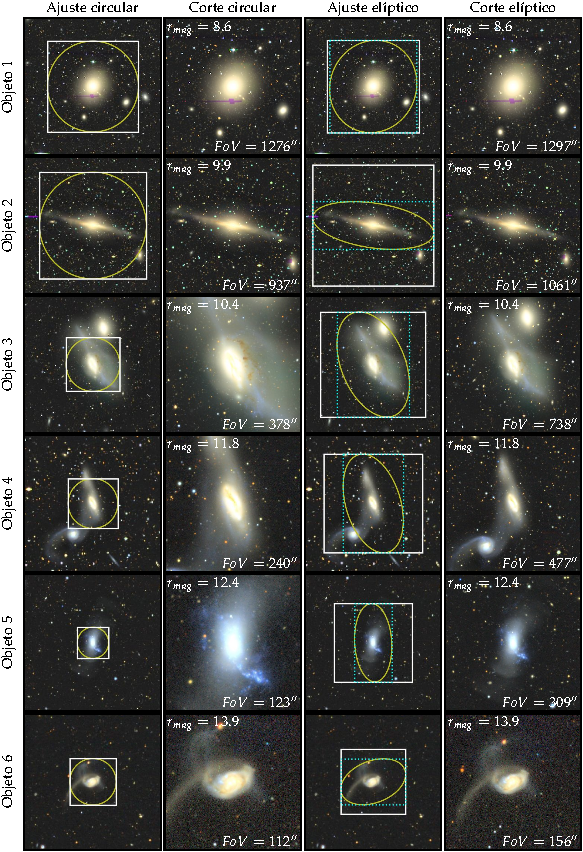
\includegraphics[width=0.89\linewidth]{notebooks/plots/stamps_crop_1.pdf}
  \caption{Ajuste do campo de visão angular para $r_{mag}$ entre 8 e 13}
  \label{fig:fov-stamps-1}
\end{figure}

\begin{figure}[!ht]
  \centering
  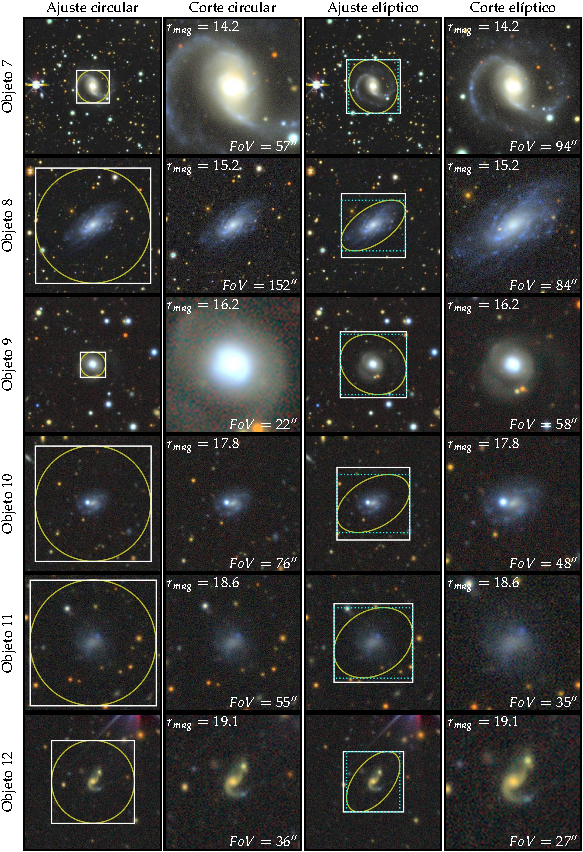
\includegraphics[width=0.89\linewidth]{notebooks/plots/stamps_crop_2.pdf}
  \caption{Ajuste do campo de visão angular para $r_{mag}$ entre 14 e 19}
  \label{fig:fov-stamps-2}
\end{figure}








\subsection{Aquisição das Imagens}
\label{sec:aquisicao-stamps}

A aquisição dos pequenos recortes de imagens astronômicas centrados em objetos específicos (stamps) do Legacy Survey por meio do serviço Hips2Fits\footnote{\url{https://alasky.cds.unistra.fr/hips-image-services/hips2fits}} \citep{aladin}, do Strasbourg Astronomical Data Center\footnote{\url{https://cds.unistra.fr}} (CDS), envolve um processo meticuloso de coleta de imagens ajustadas para um grande número de galáxias. Considerando que os campos de visão (FOVs) de cada objeto foram previamente calculados para garantir que a área da galáxia ocupe uma proporção ideal na imagem, a aquisição pode então ser automatizada, eficiente e escalável. Para realizar essa aquisição em larga escala, que pode envolver milhões de galáxias, é fundamental utilizar uma arquitetura de paralelização eficiente, como o modelo de produtor-consumidor, combinada com mecanismos de controle de taxa de requisição, mostrado na Fig. \ref{fig:stamps-sequence}.

\begin{figure}[!ht]
  \centering
  \includegraphics[width=\linewidth]{diagrams/plots/sequence.pdf}
  \caption{Diagrama de sequência da arquisição das imagens}
  \label{fig:stamps-sequence}
\end{figure}


Inicialmente, o sistema é projetado em duas camadas principais: a camada de produtores, responsáveis por gerar as requisições de imagens para cada galáxia com seu respectivo FOV, e a camada de consumidores, encarregada de processar essas requisições e armazenar os stamps retornados. No caso de uma grande quantidade de objetos, é necessário implementar várias threads que operem de forma concorrente para maximizar o desempenho e a eficiência do sistema. Os produtores criam as requisições HTTP para o Hips2Fits, especificando os parâmetros de coordenadas do objeto (como RA e Dec) e o FOV calculado. Esses parâmetros garantem que a imagem adquirida seja adequada à análise morfológica planejada.

A arquitetura paralela é gerenciada com o uso de um semáforo, um mecanismo de controle de concorrência que limita o número de requisições simultâneas feitas ao servidor Hips2Fits. Esse semáforo é configurado de acordo com a taxa de requisição máxima permitida pelo servidor, evitando sobrecarga e bloqueios temporários ou permanentes impostos pelo controle de acesso ao servidor. O semáforo atua para que um número limitado de threads possa realizar requisições ao mesmo tempo; assim, ao alcançar o limite, novas requisições aguardam até que uma thread finalize seu processo e libere o semáforo para outra requisição.

Esse modelo de produtor-consumidor com controle de taxa de requisição não apenas respeita os limites de acesso do Hips2Fits, mas também assegura uma coleta eficiente e escalável. Como cada thread pode solicitar e processar imagens independentemente, o tempo total de execução é significativamente reduzido, permitindo a aquisição dos stamps para milhões de galáxias em um tempo viável. Essa abordagem de paralelização e controle de acesso torna o sistema robusto para grandes volumes de dados, possibilitando o processamento em lotes de imagens astronômicas de forma a atender à demanda de análise em larga escala na pesquisa astronômica.





\subsection{Descrição dos Conjuntos de Dados}
\label{sec:aquisicao-descricao}

Nesta Seção, é feita uma análise, de forma agregada, sobre as propriedades físicas das galáxias dos conjuntos de dados para garantir a coerência no treinamento do modelo.

\subsubsection{Conjuntos de Treinamento, Validação e Teste}
\label{sec:aquisicao-treinamento}

Garantir que os conjuntos de treinamento, validação e teste possuam distribuições similares de magnitude (Fig. \ref{fig:conjuntos_magr}) e campo de visão angular (Fig. \ref{fig:conjuntos_fov}) é crucial para o treinamento do modelo. Distribuições consistentes asseguram que o modelo seja exposto a dados representativos durante o treinamento, prevenindo vieses que poderiam comprometer sua capacidade de generalizar para novos dados. Magnitudes diferentes podem indicar variações no brilho dos objetos, influenciando os padrões visuais extraídos pelos modelos, enquanto campos de visão angulares distintos podem alterar o contexto espacial e os detalhes observados. Desequilíbrios entre esses conjuntos podem levar a discrepâncias na avaliação, onde métricas de desempenho no conjunto de teste não refletem a eficácia real do modelo em aplicações práticas.

\begin{figure}[!ht]
  \centering
  \includegraphics[width=\linewidth]{notebooks/plots/conjuntos_magr.pdf}
  \caption{Distribuição da magnitude na banda r}
  \label{fig:conjuntos_magr}
\end{figure}


\begin{figure}[!ht]
  \centering
  \includegraphics[width=\linewidth]{notebooks/plots/conjuntos_fov.pdf}
  \caption{Distribuição do campo de visão angular}
  \label{fig:conjuntos_fov}
\end{figure}


\subsubsection{Conjunto de Inferência}
\label{sec:aquisicao-inferencia}

O conjunto de inferência é formado por aproximadamente 8 milhões de objetos. A Fig. \ref{fig:conjuntos_inferencia} mostra a distribuição espacial das galáxias, em que as cores codificam a densidade de galáxias em uma determinada região, conforme mostrado na escala.

\begin{figure}[!ht]
  \centering
  \includegraphics[width=\linewidth]{figures/similarity_footprint.pdf}
  \caption{Área de cobertura espacial do conjunto de inferência}
  \label{fig:conjuntos_inferencia}
\end{figure}


Os conjuntos de treinamento e inferência utilizados neste trabalho, composto por 400 mil e 8 milhões de imagens obtidas do DESI Legacy Survey, respectivamente, possuem uma longa durabilidade científica devido às características intrínsecas do levantamento e ao tipo de observação realizada. Como um levantamento de campo profundo e não transiente, o Legacy Survey foca na captura de objetos celestes distantes e estáticos, como galáxias e aglomerados de galáxias, que não apresentam variações significativas em escalas temporais humanas. Esses objetos, frequentemente dominados por matéria escura, são fundamentais para o estudo da evolução cósmica e da distribuição de massa no universo em larga escala. A natureza estável dessas observações permite que os dados permaneçam relevantes por décadas, fornecendo uma base sólida para análises contínuas e complementares, à medida que novos modelos de aprendizado profundo e técnicas de análise de dados são desenvolvidos. Essa durabilidade é particularmente valiosa em um contexto científico onde as demandas computacionais e as abordagens metodológicas evoluem rapidamente, garantindo que o conjunto de inferência continue a contribuir para avanços na pesquisa astronômica e cosmológica.

Esta análise encerra a seção de descrição dos dados. A seguir, serão detalhados os métodos de aprendizado profundo utilizados para o treinamento do modelo.







\section{Modelo de Aprendizagem Profunda}
\label{sec:modelo}

Neste capítulo, será explicado sobre a preparação dos dados e como fizemos o aumento artificial dos dados para obter melhores resultados na avaliação dos modelos. Em seguida, descrevemos as redes convolucionais utilizadas: VGG, Inception Resnet, EfficientNet e DenseNet. Introduzimos o conceito de (\emph{Ensemble}) e descrevemos as técnicas usadas anteriormente e que fundamentaram nossas escolhas. Em seguida, apresentamos as principais definições das redes e parâmetros utilizados neste trabalho e por fim detalhamos como foram feitas as modelagens e treinamentos dos classificadores e do nosso meta-modelo.


\begin{figure}[!ht]
  \centering
  \simpleflowdiagram{0.55}{
    Preparação das características (Seção \ref{sec:modelo-prep}),
    Aumento artificial de dados (Seção \ref{sec:modelo-dataaug}),
    Projeto da função custo (Seção \ref{sec:modelo-loss}),
    Hiperparâmetros (Seção \ref{sec:modelo-hp}),
    Treinamento (Seção \ref{sec:modelo-treinamento}),
    Métricas de Avaliação (Seções \ref{sec:metricas-votos} e \ref{sec:metricas-sim})
  }
  \caption{Fluxograma do treinamento do modelo}
  \label{fig:flow-modelo}
\end{figure}


\subsection{Preparação das Características}
\label{sec:modelo-prep}
A preparação dos dados é a etapa intuitivamente subsequente, após a aquisição (Seção \ref{sec:aquisicao}). Nessa subseção, é discutido o processamento e codificação das catacterísticas de entrada (Seção \ref{sec:modelo-prep-input}) e dos rótulos (Seção \ref{sec:modelo-prep-labels}).


\subsubsection{Preparação das Características de Entrada}
\label{sec:modelo-prep-input}
As características de entrada do modelo são as imagens do Legacy Survey DR10 (Seção \ref{sec:legacy}), obtidas pelo método descrito na Seção \ref{sec:aquisicao-stamps}. Uma etapa importante da seleção dessas características é o ajuste do campo de visão (FoV) de cada imagem. Esse ajuste determina a porcentagem que a galáxia ocupa na imagem. Visto que os píxeis referentes às galáxias são as únicas características de interesse, esse ajuste é fundamental para garantir o desempenho do modelo. Como o FoV deve ser especificado previamente, no momento da aquisição da imagem, essa etapa de ajuste do FoV já foi discutida na Seção \ref{sec:aquisicao-fov}.

O primeiro pré-processamento feito é a soma pixel a pixel no eixo dos canais RGB, produzindo uma imagem em níveis de cinza, com um único canal. Dessa forma, é mantida apenas a informação estrutural de cada galáxia. Em seguida, é feita uma normalização usando a média e o desvio padrão do lote (\texttt{BatchNormalization}).


\subsubsection{Preparação dos Rótulos}
\label{sec:modelo-prep-labels}
Os rótulos são formados pelas contagens das respostas dos voluntários do GalaxyZoo para cada galáxia. Isto é, os votos são agregados em relação a cada galáxia. As contagens de votos de cada alternativa são arranjadas na forma de vetor e os votos de diferentes campanhas são concatenados em um único vetor de votos, que é considerado o valore de referência para a estimativa das contagens de votos durante o treinamento do modelo.





\subsection{Aumento Artificial de Dados}
\label{sec:modelo-dataaug}

\begin{figure*}[!ht]
  \centering
  \includegraphics[width=\linewidth]{figures/dataaug.pdf}
  \caption{Exemplo do aumento artificial de dados em uma imagem original, mostrada no painel (a). Os painéis (b), (c), (d), (e), (f) e (g) contêm os resultados da eq. \eqref{eq:final-transformation} substituindo $M$ por diferentes combinações das transformações das eqs. \eqref{eq:aug-rot}, \eqref{eq:aug-h} e \eqref{eq:aug-v}. Em (b) $M = V$, em (c) $M = H$, em (d) $M = R(30\degree)$, em (e) $M = V R(30\degree)$, em (f) $M = H R(30\degree)$ e em (g) $M = H V R(30\degree)$.}
  \label{fig:dataaug}
\end{figure*}

Aumento artificial de dados \citep{Larry1996} é a aplicação de transformações afins nas imagens do conjunto de treinamento, por exemplo rotação, reflexão, translação e mudança de escala. As matrizes das eqs. \eqref{eq:aug-rot}, \eqref{eq:aug-h} e \eqref{eq:aug-v} definem as transformações usadas.


\begin{equation}\label{eq:aug-rot}
  R(\theta) =
  \begin{bmatrix}
    \cos(\theta) & -\sin(\theta) & 0 \\
    \sin(\theta) & \cos(\theta)  & 0 \\
    0            & 0             & 1
  \end{bmatrix}
\end{equation}


\begin{equation}\label{eq:aug-h}
  H =
  \begin{bmatrix}
    1 & 0  & 0 \\
    0 & -1 & 0 \\
    0 & 0  & 1
  \end{bmatrix}
\end{equation}


\begin{equation}\label{eq:aug-v}
  V =
  \begin{bmatrix}
    -1 & 0 & 0 \\
    0  & 1 & 0 \\
    0  & 0 & 1
  \end{bmatrix}
\end{equation}


onde $R(\theta)$ é a transformação rotação por um ângulo $\theta$,
$H$ é a transformação reflexão horizontal e $V$ é a transformação reflexão vertical, nas eqs. \eqref{eq:aug-rot}, \eqref{eq:aug-h} e \eqref{eq:aug-v}, respectivamente.

Seja $M$ a matriz das transformações combinadas, $(x, y)$ a coordenada do píxel da imagem original e $(x^*, y^*)$ a coordenada transformada do píxel, as transformações nas imagens são feitas remapeando as coordenadas dos píxeis originais aplicando uma combinação das matrizes das eqs. \eqref{eq:aug-rot}, \eqref{eq:aug-h} e \eqref{eq:aug-v} em cada píxel da imagem original usando a equação \eqref{eq:final-transformation}, onde $(t_x, t_y)$ é a coordenada do centro da imagem e as matrizes ao redor de $M$ são as matrizes translação. Isso é feito para que a transformação $M$ tenha o centro da imagem como ponto de simetria.

\begin{align} \label{eq:final-transformation}
  \begin{bmatrix}
    x^* \\
    y^* \\
    1
  \end{bmatrix}
  =
  \begin{bmatrix}
    1 & 0 & t_x \\
    0 & 1 & t_y \\
    0 & 0 & 1
  \end{bmatrix}
  \ M\
  \begin{bmatrix}
    1 & 0 & -t_x \\
    0 & 1 & -t_y \\
    0 & 0 & 1
  \end{bmatrix}
  \begin{bmatrix}
    x \\
    y \\
    1
  \end{bmatrix}
\end{align}

Além disso, ainda é aplicada uma interpolação bilinear como \emph{anti-aliasing} \citep{aliasing,bilinear}. Durante o treinamento da rede, novas imagens de entrada são geradas a cada época a partir da transformação das imagens originais. A Figura \ref{fig:dataaug} mostra a imagem original, no painel (a), e diversas transformações, nos demais painéis, aplicadas substituindo $M$ da equação \eqref{eq:final-transformation} por combinações (multiplicação matricial) das transformações das eqs. \eqref{eq:aug-rot}, \eqref{eq:aug-h} e \eqref{eq:aug-v}. Tais transformações não mudam a interpretação da classe da imagem original, pois o espaço visual é invariante a elas. Logo, o objetivo de aplicar estas transformações nas imagens de entrada da rede é deixar que o algorítmo infira tal invariância, criando, assim, uma ``noção'' do espaço visual, o que resulta no aumento do potencial de generalização da rede \citep{Simard2003,CholletBook}. Frequentemente são relatados bons resultados com o uso desta técnica \citep{EfficientNetEx01,EfficientNetEx02,CNNEx04}, principalmente quando existe grande similaridade entre as classes.






% \subsection{Preparação dos dados}
% \label{section:preparacao}

% O pré-processamento é a preparação das imagens para serem usadas pelo modelo, ou seja, é a transformação dos dados não processados em dados prontos para entrada na rede. Isso envolve representar as imagens por matrizes multidimensionais, onde cada elemento da matriz representa um pixel da imagem, e aplicar algumas transformações, especificadas a seguir.

% \subsubsection{Agrupamento das bandas para confecção das imagens RGB}

% Como as imagens do S-PLUS foram obtidas em 12 bandas fotométricas (listadas em \citep{splus}), para representá-las no sistema de cor RGB fizemos o seguinte mapeamento: em R colocamos as 4 bandas vermelhas r\_SDSS, i\_SDSS, J0861 e z, em G as bandas g\_SDSS J0515 e J0660 e em B as cinco bandas mais azuis u\_JAVA, J0373, J0395, J0410 e J0430 (as características destes filtros são dadas na Tabela 1 de \citep{splus}). Na combinação de bandas em cada canal, foi feita uma soma simples dos valores dos píxeis. Depois de reduzidas a três bandas, as imagens são usadas como entrada do programa Trilogy\citep{coe2012clash}\footnote{\url{https://www.stsci.edu/~dcoe/trilogy/Intro.html}}.

% \subsubsection{ImageNet}

% Como já mostrado em trabalhos anteriores, a inicialização dos pesos provenientes de uma rede pré-treinada usando a base de dados \emph{ImageNet}\footnote{\url{http://www.image-net.org/}} traz uma grande melhoria na precisão dos resultados da classificação. Essa base de dados possui milhões de imagens de objetos do cotidiano e já foi utilizada especificamente para a classificação de objetos astronômicos (veja por exemplo \citep{bom2021}), com excelentes resultados.

% O uso deste dataset para pré-treinamento respeitou o pré-processamento utilizado originalmente pelos autores de cada rede, este procedimento este foi crucial para garantir um fit competitivo, isto é, no \textit{benchmarking} original destas redes para os dados da \emph{ImageNet}. Para a rede VGG16 (Seção \ref{section:vgg}), a ordem das bandas foi trocada de RGB para BGR, e cada banda foi centrada em zero em relação à \emph{ImageNet}, sem escalonamento, ou seja, os píxeis de cada banda tiveram o valor da média da respectiva banda \emph{ImageNet} subraído. Para a rede InceptionResNetV2 (Seção \ref{section:inceptionresnetv2}), os píxeis de entrada foram escalonados entre -1 e 1 em relação a amostra de treino. Para a rede EfficientNet (Seção \ref{section:efficientnet}), os píxeis de entrada foram escalonados entre 0 e 1 em relação à amostra de treino. E, para a rede DenseNet (Seção \ref{section:densenet}), os píxeis de entrada foram escalonados entre 0 e 1 e cada banda foi padronizada em relação à \emph{ImageNet}, isto é, os píxeis de cada banda tiveram o valor da média subtraído e o resultado foi dividido pelo desvio padrão da distribuição da respectiva banda da \emph{ImageNet}.

% \begin{figure*}[!ht]
%   \centering
%   \includegraphics[width=\textwidth]{figures/arch.pdf}
%   \caption{Diagrama que descreve a arquitetura da rede. Da esquerda para a direita, as 12 imagens de cada banda são agrupadas em uma única imagem RGB (Seção \ref{section:preparacao}), que é a entrada dos classificadores indidviduais. Estes classificadores (Seção \ref{section:classificador}) têm a função de extrair características visuais da imagem e retornar a probabilidade de ser elíptica ou espiral. O meta-modelo (Seção \ref{section:meta-modelo}) tem a função de combinar as predições dos classificadores em uma única predição final mais robusta.}
%   \label{fig:arch}
% \end{figure*}






\subsection{Função de Custo}
\label{sec:modelo-loss}


\subsubsection{Distribuição Multinomial}
\label{sec:modelo-multi}

A distribuição multinomial \citep{distbook-multinomial} é uma generalização da distribuição binomial \citep{distbook-binomial} que descreve o comportamento de um experimento discreto onde cada tentativa resulta em um de $k$ possíveis resultados mutuamente exclusivos.

Supondo que um experimento é repetido $n$ vezes, e que a probabilidade de cada resultado específico $i$, para $i=1,2,\dots,k$, seja $p_i$, com $\sum_{i=1}^k p_i = 1$. A distribuição multinomial caracteriza a probabilidade conjunta de observar cada um dos $k$ resultados um número específico de vezes ($x_1, x_2,\dots, x_k$), onde $\sum_{i=1}^k x_i = n$. A função de probabilidade associada é definida pela eq. \eqref{eq:multinomial}, onde \( x_i \geq 0 \) representa a contagem de ocorrências para cada categoria \( i \).

\begin{equation}\label{eq:multinomial}
  P(X_1 = x_1, X_2 = x_2, \dots, X_k = x_k) = \frac{n!}{x_1! x_2! \cdots x_k!} \prod_{i=1}^k p_i^{x_i}
\end{equation}

A distribuição multinomial \citep{seber2015-multi} é amplamente utilizada em aplicações de aprendizado de máquina e estatística, como na modelagem da transmissão de Dengue \citep{wang2025}, na predição de cotação de mercado \citep{nevasalmi2020} e na análise de tráfego aéreo \citep{torres2023}. Uma de suas principais aplicações é em modelagem de eventos categóricos \citep{kibriya2004,luo2021}. Por exemplo, em tarefas de classificação multiclasse, onde o objetivo é prever a probabilidade de uma amostra pertencer a uma entre várias categorias, a distribuição multinomial é usada para modelar a saída do modelo. Um exemplo prático é o uso em algoritmos como o Naive Bayes Multinomial \citep{kalcheva2023,jiang2016}, amplamente empregado em problemas de classificação de texto \citep{odeh2022,kan2005}, como análise de sentimentos \citep{saravanan2023} e categorização de documentos. Neste contexto, as palavras em um documento são tratadas como eventos que seguem uma distribuição multinomial.

% Outra aplicação significativa é no modelamento de linguagens probabilísticas, como em modelos n-grama usados para processamento de linguagem natural (NLP). Nesses modelos, a distribuição multinomial é usada para representar a probabilidade de coocorrência de palavras em sequência. Além disso, na estimação de tópicos em conjuntos de documentos, como no algoritmo Latent Dirichlet Allocation (LDA), a distribuição multinomial é usada para modelar a distribuição de palavras em tópicos e tópicos em documentos.

% No campo de aprendizado profundo, a distribuição multinomial aparece em camadas de saída de redes neurais voltadas para classificação multiclasse, onde a função softmax é usada para transformar as saídas da rede em probabilidades que seguem uma distribuição multinomial. Esse uso é especialmente prevalente em problemas como reconhecimento de imagens e detecção de objetos.

% Por fim, a distribuição multinomial também desempenha um papel importante em amostragem e inferência estatística. Em métodos como amostragem Gibbs e Markov Chain Monte Carlo (MCMC), é comum gerar amostras a partir de distribuições multinomiais para explorar o espaço de parâmetros em modelos probabilísticos complexos.


\subsubsection{Distribuição de Dirichlet}
\label{sec:modelo-dir}

A distribuição Dirichlet \citep{distbook-dirichlet} é uma distribuição de probabilidade multivariada contínua definida no simplex \( k \)-dimensional, sendo uma generalização da distribuição Beta \citep{distbook-beta} para múltiplas dimensões. Ela é frequentemente utilizada para modelar distribuições de probabilidade sobre proporções, em que cada elemento do vetor de variáveis aleatórias representa uma fração de um todo e, portanto, suas somas totalizam 1.

Dada uma variável aleatória \( \vec{X} = (X_1, X_2, \dots, X_k) \) que segue uma distribuição Dirichlet com parâmetro de concentração \( \vec{\alpha} = (\alpha_1, \alpha_2, \dots, \alpha_k) \) para uma quantidade $k$ de categorias, a função de densidade de probabilidade é definida pela eq. \eqref{eq:dirichlet}, onde \( B(\vec{\alpha}) \) é a função beta multivariada, definida na eq. \eqref{eq:dirichlet-B}, e \( \Gamma(\cdot) \) representa a função gama \citep{distbook-gamma}. O parâmetro \( \alpha_i \) controla a concentração da probabilidade ao redor das categorias: valores maiores de \( \alpha_i \) indicam maior densidade de probabilidade associada à categoria correspondente.

\begin{equation}\label{eq:dirichlet}
  P(\vec{X} | \vec{\alpha}) = \frac{1}{B (\vec{\alpha})} \prod_{i=1}^k X_i^{\alpha_i - 1}
\end{equation}

\begin{equation}\label{eq:dirichlet-B}
  B(\vec{\alpha}) = \frac{\prod_{i=1}^k \Gamma(\alpha_i)}{\Gamma\left(\sum_{i=1}^k \alpha_i\right)}
\end{equation}


Em aprendizado de máquina, a distribuição Dirichlet possui aplicações importantes em problemas que envolvem modelagem de distribuições de probabilidade sobre categorias. Um exemplo clássico é na modelagem de misturas probabilísticas, como no algoritmo Latent Dirichlet Allocation (LDA; \citealp{lda}), amplamente utilizado para análise de tópicos em grandes corpora de texto \citep{jelodar2019}. No LDA, a distribuição Dirichlet é usada como uma distribuição a priori para representar a probabilidade de tópicos em documentos e a probabilidade de palavras em tópicos, fornecendo uma forma eficiente de capturar relações semânticas latentes \citep{canini2009}.

% Além disso, a distribuição Dirichlet é usada em inferência bayesiana, especialmente como conjugado da distribuição multinomial. Em tarefas como classificação multiclasse, a combinação da distribuição Dirichlet com a multinomial permite a atualização eficiente das probabilidades a priori para a modelagem de eventos categóricos. Esse mecanismo é essencial em algoritmos de aprendizado supervisionado que se baseiam em pressupostos probabilísticos, como o Naive Bayes Multinomial.

% Outro campo de aplicação da distribuição Dirichlet é o **aprendizado de misturas**, onde modelos como o Dirichlet Process Mixture Model (DPMM) usam essa distribuição para lidar com dados agrupados, mas com um número potencialmente infinito de clusters. Essa característica é particularmente útil em problemas não supervisionados, onde o número de classes ou clusters não é conhecido a priori.

% Na **simulação e geração de dados sintéticos**, a distribuição Dirichlet é frequentemente empregada para gerar distribuições de probabilidades em modelos de simulação. Por exemplo, em aprendizado por reforço, ela pode ser usada para modelar incertezas nas probabilidades de transição entre estados em ambientes estocásticos.

% Por fim, a distribuição Dirichlet também desempenha um papel em métodos de regularização. Em problemas de otimização envolvendo distribuições de probabilidades, ela pode ser usada para impor uma estrutura probabilística bem definida, evitando soluções degeneradas ou com concentração excessiva de probabilidades em poucas categorias.

% Em resumo, a distribuição Dirichlet é uma ferramenta central para modelar proporções e distribuições categóricas em múltiplas áreas do aprendizado de máquina, oferecendo uma base teórica sólida para lidar com problemas envolvendo incertezas e relações probabilísticas complexas.




\subsubsection{Distribuição Dirichlet-Multinomial}
\label{sec:modelo-dir-multi}

A distribuição Dirichlet-multinomial \citep{distbook-dirichlet} é uma distribuição de probabilidade discreta que combina as propriedades da distribuição multinomial (Seção \ref{sec:modelo-multi}) e da distribuição Dirichlet (Seção \ref{sec:modelo-dir}). Ela é usada para modelar processos em que as probabilidades das categorias em uma distribuição multinomial são, elas mesmas, amostras de uma distribuição Dirichlet. Isto é, a distribuição Dirichlet é usada como distribuição a priori para estimar os parâmetros da distribuição multinomial. Essa estrutura permite incorporar incertezas sobre as probabilidades subjacentes das categorias.

Formalmente, dado um vetor \( \vec{\theta} = (\theta_1, \theta_2, \dots, \theta_k) \) de probabilidades categóricas que segue uma distribuição Dirichlet com parâmetro \( \vec{\alpha} = (\alpha_1, \alpha_2, \dots, \alpha_k) \), e uma distribuição multinomial condicional sobre \( \vec{\theta} \), a probabilidade conjunta da distribuição Dirichlet-multinomial é expressa na eq. \eqref{eq:dirichlet-multinomial}, onde \( n = \sum_{i=1}^k x_i \) é o número total de experimentos, e \( x_i \) representa o número de ocorrências da \( i \)-ésima categoria.

\begin{equation}\label{eq:dirichlet-multinomial}
  P(X_1 = x_1, X_2 = x_2, \dots, X_k = x_k) = \frac{\Gamma\left(\sum_{i=1}^k \alpha_i\right)}{\Gamma\left(\sum_{i=1}^k \alpha_i + n\right)} \prod_{i=1}^k \frac{\Gamma(x_i + \alpha_i)}{\Gamma(\alpha_i) \, x_i!}
\end{equation}




\subsubsection{Função de Custo e Função de Perda}
\label{sec:modelo-loss-cost}

A função de perda (\emph{loss function}) e a função de custo (\emph{cost function}) têm papéis relacionados, mas distintos. A primeira avalia o erro do modelo em uma única amostra, medindo a discrepância entre a predição do modelo e o valor esperado. Já a segunda, é uma agregação da primeira, geralmente calculada como a média ou soma das perdas sobre todo o conjunto de treinamento, representando o desempenho global do modelo. %Isto é, enquanto a loss function opera em nível de exemplo individual, a cost function fornece uma visão geral para otimizar o modelo durante o treinamento.

% A escolha da função de perda possui impacto direto na capacidade preditiva do modelo. Por isso, escolhemos uma função de custo

% As informações morfológicas sobre as galáxias são obtidas pelo projeto GalaxyZoo, que consistem nos votos de voluntários para diversas perguntas sobre suas características visuais, como a orientação espacial, a presença de bojo, a quantidade de braços espirais, etc. Então, considerando a origem dos dados, a distribuição Dirichlet-multinomial (Seção \ref{sec:modelo-dir-multi}) foi escolhida como função de custo.

A função de perda de uma pergunta $q$ é calculada a partir da distribuição Dirichlet-Multinomial, conforme a eq. \eqref{eq:loss}.

\begin{equation}\label{eq:loss}
  \mathcal{L}_q = \int\text{Multi}(\vec{k}|\vec{\rho}, N) \text{Dirichlet}(\vec{\rho}|\vec{\alpha})d\vec{\rho}
\end{equation}

Já o valor da perda de um exemplo é a soma das perdas de cada questão $q$, conforme a eq. \eqref{eq:log_loss}.

\begin{equation}\label{eq:log_loss}
  \log \mathcal{L} = \sum_q \mathcal{L}_q(\vec{k_q}, N_q, \vec{f_q^w})
\end{equation}

Existem duas formas recorrentes de agregar as perdas dos exemplos para calcular o custo total do modelo: calcular a soma  ou a média. Nesse trabalho, a função de custo é definda como a soma de todas as perdas de cada exemplo do conjunto de dados, conforme eq. \eqref{eq:cost}.

\begin{equation}\label{eq:cost}
  J = \sum_i \log \mathcal{L}_i
\end{equation}


% ### Propriedades e Intuição
% A distribuição Dirichlet-multinomial é uma extensão prática da distribuição multinomial porque incorpora variabilidade adicional na estimativa das probabilidades \( \boldsymbol{\theta} \). Isso a torna ideal para modelar dados categóricos onde há incerteza ou variabilidade na distribuição subjacente. Como tal, ela é frequentemente descrita como uma multinomial com parâmetros aleatórios seguindo uma Dirichlet.

% ### Aplicações em Aprendizado de Máquina
% No campo de aprendizado de máquina, a distribuição Dirichlet-multinomial possui aplicações significativas em **modelagem probabilística** e **inferência bayesiana**. Uma de suas utilizações mais comuns é na modelagem de fenômenos categóricos em que a frequência das categorias varia entre diferentes conjuntos de dados ou instâncias.

% #### 1. **Latent Dirichlet Allocation (LDA)**
% Na análise de tópicos, a Dirichlet-multinomial é usada para modelar a distribuição das palavras em documentos. Cada documento é tratado como uma realização de uma multinomial, cujas probabilidades de categorias (palavras) são amostras de uma Dirichlet. Essa abordagem permite capturar as variações de distribuição de palavras entre tópicos, sendo central para algoritmos como o **Latent Dirichlet Allocation (LDA)**, amplamente utilizado em **processamento de linguagem natural**.

% #### 2. **Inferência Bayesiana em Classificação Multiclasse**
% A Dirichlet-multinomial é o modelo conjugado da distribuição multinomial em inferência bayesiana. Em problemas de **classificação multiclasse**, ela é usada para modelar a incerteza nas estimativas das probabilidades das classes, particularmente em cenários de aprendizado supervisionado onde os dados de treinamento são limitados.

% #### 3. **Modelagem de Contagens e Variabilidade**
% Problemas que envolvem dados de contagem, como análise de redes sociais, preferências de usuários ou frequências de eventos em sistemas distribuídos, frequentemente apresentam superdispersão (variância maior que a média). A Dirichlet-multinomial é adequada para modelar essa superdispersão, fornecendo uma alternativa robusta à multinomial tradicional.

% #### 4. **Misturas de Modelos e Clusterização**
% Na clusterização, especialmente em métodos baseados em misturas, como o **Dirichlet Process Mixture Models (DPMM)**, a Dirichlet-multinomial pode ser usada para modelar distribuições de contagens em diferentes clusters. Esse uso é especialmente relevante em problemas de agrupamento não supervisionado.

% #### 5. **Geração de Dados Sintéticos**
% A distribuição Dirichlet-multinomial também é amplamente utilizada para gerar dados categóricos sintéticos que incorporam incertezas ou variabilidades realistas, sendo valiosa em experimentos controlados e validações de algoritmos.

% ### Conclusão
% A distribuição Dirichlet-multinomial é uma ferramenta poderosa para modelar processos categóricos que exibem variabilidade nas probabilidades subjacentes. Sua capacidade de capturar incertezas intrínsecas torna-a essencial em uma ampla gama de aplicações, especialmente na modelagem de tópicos, inferência bayesiana e análise de dados de contagem. No aprendizado de máquina, ela desempenha um papel central ao lidar com problemas onde a variabilidade das distribuições subjacentes é uma característica fundamental dos dados.




\subsection{Hiperparâmetros}
\label{sec:modelo-hp}

Nesta seção descrevemos as definições dos principais conceitos, no contexto de deep learning, que serão úteis para o entendimento dos métodos aqui utilizados. A função de ativação, função de custo, o otimizador, o learning rate, o número de épocas, além do número de camadas dos modelos, são importantes parâmetros responsáveis pela contrução do modelo definido a seguir.

\begin{description}
  \item[Função de ativação] \hfill \\
        A função de ativação é responsável por adicionar não-linearidade à rede. Sem ela, a saída de uma camada seria apenas uma transformação linear dos dados de entrada e a rede não seria beneficiada pelo empilhamento de diversas camadas lineares, pois isso não aumentaria o espaço de hipóteses. Logo, a função de ativação viabiliza representações mais complexas da rede, uma vez que define a complexidade de um modelo e, consequentemente, sua capacidade de generalização \citep{CholletBook}. Neste trabalho, a função $\textrm{ReLU}(x) := \textrm{max}(0, x)$ é usada nas camadas densas dos classificadores, a equação tangente hiperbólica é usada nas camadas densas do meta-modelo e a função Softmax \citep{Bridle1990} foi usada na última camada, tanto dos classificadores quanto do meta-modelo.

  \item[Otimizador] \hfill \\
        O otimizador é um algorítmo iterativo com objetivo de minimizar a função de custo. Uma escolha típica é o método de gradiente descente e suas demais variações. Este tipo de algoritmo tem um parâmetro livre relacionado ao passo da iteração conhecido como taxa de aprendizado ou \textit{learning rate}. Neste trabalho foram testados diversos algoritmos considerados como estado-da-arte dos otimizadores como Adam \citep{Adam}, NAdam \citep{NAdam}, RAdam \citep{RAdam} e RMSprop \citep{RMSprop}.

  \item[Número de Épocas] \hfill \\
        O Número de épocas se referem a quantidade de vezes que o dataset de treino foi utilizado completamente no processo de otimização iterativa da função de custo. Um número de épocas adequado é necessário para que a função de custo seja minimizada.

  \item[Tamanho do Batch] \hfill \\
        O processo de otimização acontece em batches, cada iteração para minimizar a função custo é realizada com um número fixo de amostras, quando todas as amostras de treino são utilizadas se completa uma época.

  \item[Unidades de neurônios na última camada]
        \hfill \\
        A última camada da rede antes da camada de saída é responsável por condensar toda a informação extraída da rede para o processo de classificação final. Por esta razão, a quantidade de neurônios nessa camada pode ser particularmente sensível para a performance da rede. Neste trabalho utilizamos diferentes valores de neurônios para encontrar a quantidade que pode gerar a melhor performance.

  \item[Dropout]
        \hfill \\
        \emph{Dropout} \citep{dropout} é uma técnica de regularização muito utilizada em redes neurais por seu bom desempenho e baixo custo computacional. Aplicar esta regularização em uma camada consiste em eliminar aleatoriamente uma taxa dos neurônios de saída desta camada durante o treinamento, sendo geralmente escolhido um valor entre 0.2 e 0.5 para esta taxa \citep{CholletBook}.
\end{description}












\subsection{Arquitetura de Rede Neural}
\label{sec:arch}

\subsubsection{Visual Geometry Group Networks}
\label{sec:vgg}
A família de arquiteturas Visual Geometry Group Networks (VGGNets) \citep{VGG16} foi criada durante a competição de classificação de imagens \textit{Large Scale Visual Recognition Challenge} \citep{ILSVRC15}. Ela se destaca por estar entre as primeiras redes a adotar, com sucesso, o escalamento em profundidade (quantidade de camadas) para aumentar o desempenho na classificação de imagens usando redes convolucionais. Neste trabalho, consideramos a arquitetura VGG16, que já foi usada em diversas tarefas de classificação, como a classificação de software malicioso \citep{VGG16Ex01}, de plantas \citep{VGG16Ex02} e de tumores cerebrais \citep{VGG16Ex03}.

\subsubsection{InceptionResNetV2}
\label{sec:inceptionresnetv2}
A arquitetura InceptionResNetV2 \citep{InceptionResNetv2} usa os blocos Inception, que são convoluções fatorizadas, introduzidos em \citep{Inception}, motivada pela construção de redes mais profundas com um menor custo computacional e menor overfitting, com a adição de conexões residuais \citep{ResNet} motivada pelo problema de dissipação do Gradiente (\textit{vanishing gradients}). Isso permite treinar redes profundas com maior acurácia e mais rápido. Esta arquitetura já foi usada, por exemplo, para classificação de imagens de satélite \citep{InceptionResNetV2Ex01}, de ultrasonografia \citep{InceptionResNetV2Ex02} e de células cancerígenas \citep{InceptionResNetV2Ex03}.

\subsubsection{EfficientNet}
\label{sec:efficientnet}
A arquitetura EfficientNet \citep{EfficientNet} foi desenvolvida como uma resposta à questão de como escalar modelos de convolução. Foram considerados três diferentes aspectos: profundidade, largura e resolução da imagem de entrada. Em vez de dimensionar cada aspecto manualmente, o modelo implementa um escalonamento composto que equilibra os aspectos para obter melhor desempenho, com isso a rede consegue uma alta acurácia usando muito menos parâmtros e operações de ponto flutuante por segundo (\emph{FLOPS}). Esta rede já foi usada na classificação de doenças em vegetais \citep{EfficientNetEx03}, eletrocardiogramas \citep{EfficientNetEx01} e cristalização de proteínas \citep{EfficientNetEx02}.

\subsubsection{DenseNet}
\label{sec:densenet}
A rede DenseNet \citep{DenseNet} também usa conexões residuais que conectam cada camada a todas as outras camadas seguintes, o que reduz ainda mais o número de parâmetros na rede sem perda significativa da precisão. O uso desta rede incluem predição do mapa de contato de proteínas \citep{DenseNetEx02}, classificação de músicas \citep{DenseNetEx05}, câncer de mama \citep{DenseNetEx01} e esclerose múltipla \citep{DenseNetEx03}.


\subsubsection{Escolha da Arquitetura}
\label{sec:escolha-arch}
Todas as arquiteturas convolucionais mencionadas nessa seção foram testadas e a arquitetura que teve melhor desempenho na predição dos votos dos voluntários foi escolhida. O processo de treinamento e avaliação está descrito na seção seguinte.



\subsection{Treinamento}
\label{sec:modelo-treinamento}

O treinamento de modelos de aprendizado profundo é um processo complexo que envolve a escolha de uma arquitetura adequada e a definição de hiperparâmetros que otimizem o desempenho do modelo em um conjunto de dados específico. A técnica de treinamento automatizado (AutoML; \citealp{automl}), mostrada na Fig. \ref{fig:treinamento}, facilita esse processo de seleção de hiperparâmetros e configurações de treinamento. Neste trabalho, foi utilizada uma abordagem que se mostrou eficaz nesse contexto: os algoritmos Multi-Objective Tree-structured Parzen Estimator (MOTPE; \citealp{motpe}) e HyperBand (HB; \citealp{hyperband}), disponíveis na biblioteca Optuna\footnote{\url{https://optuna.org}} \citep{optuna}, para a otimização de múltiplos objetivos simultaneamente.

\begin{figure}[!ht]
  \centering
  \includegraphics[width=\linewidth]{figures/treinamento.png}
  \caption{Treinamento do modelo}
  \label{fig:treinamento}
\end{figure}

O treinamento com AutoML utilizando o MOTPE envolve diversas etapas estruturadas, desde a configuração inicial do espaço de busca dos hiperparâmetros até a avaliação iterativa dos modelos. A seguir, descrevem-se as principais etapas do processo:

\begin{enumerate}
  \item \textbf{Definição do Espaço de Busca dos Hiperparâmetros:}
        Inicialmente, define-se um espaço de busca para os hiperparâmetros do modelo, que pode incluir a taxa de aprendizado, número de camadas, número de neurônios por camada, taxas de dropout, tipos de ativação, otimizadores, entre outros. Para cada hiperparâmetro, especificam-se limites, distribuições ou valores discretos que serão explorados pelo algoritmo.

  \item \textbf{Criação da Função de Objetivo:}
        A função de objetivo é o núcleo do processo de otimização. Ela recebe uma configuração de hiperparâmetros como entrada, treina e avalia o modelo utilizando essa configuração, e retorna uma ou mais métricas de desempenho que serão otimizadas. No caso do MOTPE, que é multiobjetivo, é possível considerar métricas conflitantes, como minimizar o erro de validação enquanto reduz o tempo de treinamento.

  \item \textbf{Treinamento Iterativo com Amostragem Bayesiana:}
        O MOTPE utiliza um modelo probabilístico para guiar a busca por configurações promissoras. Ele avalia iterativamente as combinações de hiperparâmetros, ajustando o modelo probabilístico com base nos resultados obtidos em iterações anteriores. Isso permite uma exploração mais eficiente do espaço de busca, concentrando-se em áreas com maior probabilidade de melhorar o desempenho.

  \item \textbf{Validação e Regularização:}
        Cada configuração de hiperparâmetros é validada em um conjunto de validação separado para garantir que o modelo não esteja superajustando os dados de treinamento. Além disso, o uso de técnicas como early stopping e regularização (L2 ou dropout) é integrado ao treinamento para evitar overfitting.

  \item \textbf{Seleção do Melhor Modelo:}
        Após um número predefinido de iterações ou ao atingir um critério de parada, o AutoML seleciona a configuração de hiperparâmetros que apresenta o melhor desempenho médio em relação às métricas otimizadas. No caso de otimização multiobjetivo, a solução é escolhida com base no conceito de fronteira de Pareto.
\end{enumerate}

A Tabela \ref{tab:hps} sumariza os hiperparâmetros otimizados pelo MOTPE. Nela são mostrados os intervalos de busca para cada hiperparâmetro, bem como a distribuição utilizada para cada um deles.


\begin{table}[!ht]
  \centering
  \caption{Intervalos de busca dos hiperparâmetros otimizados com o MOTPE}
  \label{tab:hps}
  \begin{tabular}{lll}
    \toprule
    Hiperparâmetro            & Distribuição     & Intervalo de Busca              \\
    \midrule
    Arquitetura               & Categórica       & \{VGG, IRV2, EffNet, DenseNet\} \\
    Taxa de aprendizado       & Log-Uniforme     & $[10^{-5}, 10^{-1}]$            \\
    Número de camadas ocultas & Int-Uniforme     & $[0, 5]$                        \\
    Neurônios por camada      & Int-Uniforme     & $[32, 512]$                     \\
    Taxa de dropout           & Uniforme         & $[0.1, 0.5]$                    \\
    Otimizador                & Categórica       & \{Adam, NAdam, SGD, RMSprop\}   \\
    Batch size                & Int-Log-Uniforme & $[16, 256]$                     \\
    Peso da regularização L2  & Log-Uniforme     & $[10^{-5}, 10^{-2}]$            \\
    Função de ativação        & Categórica       & \{ReLU, Leaky ReLU, ELU\}       \\
    \bottomrule
  \end{tabular}
\end{table}




\subsection{Métricas de Avaliação da Predição dos Votos}
\label{sec:metricas-votos}

As métricas aqui utilizadas baseiam-se no erro ou acerto na associação dos objetos às classes pelo modelo. Para relacionar a probabilidade calculada pelo modelo à classe, é definido um limiar de discriminação, que é a probabilidade mínima para que um exemplar pertença à uma classe. Para o cálculo das métricas, foi considerado um de limiar de 0.5.

\subsubsection{Matriz de Confusão}
\label{sec:metricas-confusao}

A matriz de confusão consiste em um modelo tabular que cruza métricas de predição e referência, sendo comumente usada para avaliar a qualidade preditiva de modelos de aprendizagem de máquina. A Tabela \ref{tab:cm} mostra um esquema desta matriz para o caso de classificação binária (apenas duas classes). A análise para mais classes pode ser feita isolando uma classe positiva por vez e reduzindo o problema a multiplas classificações binárias.

\begin{table}[!ht]
  \centering
  \caption{Estrutura da matriz de confusão para classificação binária}
  \label{tab:cm}
  \begin{tabular}{lll}
    \toprule
    {}                          & \multicolumn{2}{c}{Predição}                            \\
    \midrule
    \multirow{2}{*}{Verdadeiro} & Verdadeiro Positivo (VP)     & Falso Negativo (FN)      \\
    {}                          & Falso Positivo (FP)          & Verdadeiro Negativo (VN) \\
    \bottomrule
  \end{tabular}
\end{table}

A seguir, são definidas cada uma das métricas usadas para montar a matriz de confusão.

\begin{itemize}
  \item Verdadeiro Positivo (VP): O modelo prevê uma instância verdadeira corretamente
  \item Verdadeiro Negativo (VN): O modelo prevê uma instância negativa corretamente
  \item Falso Positivo (FP): O modelo prevê uma instância positiva, mas, na verdade, é negativa. Este é o erro tipo I, que consiste em rejeitar a hipótese nula quando ela é verdadeira.
  \item Falso Negativo (FN): O modelo prevê uma instância negativa, mas, na verdade, é positiva. Este é o erro tipo II, em estatística, que consiste na falha em rejeitar a hipótese nula quando ela é falsa.
\end{itemize}



\subsubsection{Acurácia}
\label{sec:metricas-acc}

A acurácia é uma métrica que mede a proporção de predições corretas em relação ao total de instâncias avaliadas. Ela é definida como indicado na eq. \ref{eq:acc}.

\begin{equation}\label{eq:acc}
  \text{Acurácia} = \frac{\text{VP} + \text{VN}}{\text{VP} + \text{VN} + \text{FP} + \text{FN}}
\end{equation}



\subsubsection{Precisão}
\label{sec:metricas-precisao}

A precisão avalia a proporção de exemplos classificados como positivos que são realmente positivos, conforme a eq. \eqref{eq:precisao}, sendo particularmente importante em cenários onde o custo de falsos positivos é alto.

\begin{equation}\label{eq:precisao}
  \text{Precisão} = \frac{\text{VP}}{\text{VP} + \text{FP}}.
\end{equation}




\subsubsection{Revocação}
\label{sec:metricas-revocacao}

A revocação, também conhecida como sensibilidade ou taxa de verdadeiros positivos, mede a capacidade do modelo de identificar corretamente os exemplos positivos, conforme a eq. \eqref{eq:recall}, sendo principalmente útil em contextos onde a identificação de todos os exemplos positivos é crucial

\begin{equation}\label{eq:recall}
  \text{Revocação} = \frac{\text{VP}}{\text{VP} + \text{FN}}.
\end{equation}




\subsubsection{F1-Score}
\label{sec:metricas-f1}

O F1-score é a média harmônica entre precisão e revocação, sendo usado como uma métrica de equilíbrio entre essas duas dimensões, conforme a eq. \eqref{eq:f1}. Esta métrica é útil quando há uma compensação entre precisão e revocação, como em cenários com classes desbalanceadas, pois fornece uma medida única que leva em conta ambos os aspectos. Valores de \( F1 \) próximos de 1 indicam que o modelo apresenta um bom equilíbrio entre os dois fatores.

\begin{equation}\label{eq:f1}
  F1 = 2 \cdot \frac{\text{Precisão} \cdot \text{Revocação}}{\text{Precisão} + \text{Revocação}}
\end{equation}






\subsection{Métricas de Avaliação da Similaridade}
\label{sec:metricas-sim}

A recuperação de imagens baseada em embeddings gerados por modelos de aprendizado de máquina envolve a comparação de vetores em um espaço latente para determinar a semelhança ou dissimilaridade entre as representações das imagens. Para isso, são amplamente utilizadas métricas de distância ou similaridade, como similaridade do cosseno (Seção \ref{sec:metricas-cos}), produto interno (Seção \ref{sec:metricas-dot}), distância L1 (Seção \ref{sec:metricas-l1}) e distância L2 (Seção \ref{sec:metricas-l2}). Essas métricas capturam diferentes aspectos das relações entre os embeddings e são escolhidas com base nas características do espaço latente e nos objetivos do sistema. Ademais, nessa Seção, também é definida a métrica que quantifica a capacidade preditiva da tarefa de recuperação por similaridade visual na Seção \ref{sec:metricas-map}.


\subsubsection{Distância do Cosseno}
\label{sec:metricas-cos}

A similaridade do cosseno mede o ângulo entre dois vetores no espaço vetorial, desconsiderando suas magnitudes. Ela é amplamente usada em tarefas de recuperação de imagens e processamento de linguagem natural, pois é invariável à escala dos vetores, o que é útil em embeddings que capturam informações relativas às direções no espaço latente.

Formalmente, ela é definida pela eq. \eqref{eq:cos}, onde \( \mathbf{u} \cdot \mathbf{v} \) é o produto interno dos vetores \( \mathbf{u} \) e \( \mathbf{v} \), e \( \|\mathbf{u}\| \) e \( \|\mathbf{v}\| \) são suas normas. Valores de $\cos(\theta)$ variam entre -1 e 1, onde 1 indica vetores perfeitamente alinhados (paralelos), -1 indica vetores opostos, e 0 indica vetores ortogonais. Já a similaridade do cosseno é mais parecida com outras métricas de distância, pois parte do princípio que coisas próximas possuem valores de distância pequenos, variando de 0 a 2. Quanto mais próximo de zero, mais similar.

\begin{equation}\label{eq:cos}
  \text{Similaridade do Cosseno} = 1-\cos(\theta) = 1-\frac{\mathbf{u} \cdot \mathbf{v}}{\|\mathbf{u}\| \|\mathbf{v}\|}
\end{equation}



\subsubsection{Produto Interno}
\label{sec:metricas-dot}

O produto interno é uma métrica simples que mede a projeção de um vetor sobre outro, conforme a eq. \eqref{eq:dot}, onde \( u_i \) e \( v_i \) são as componentes correspondentes dos vetores \( \mathbf{u} \) e \( \mathbf{v} \). Diferentemente da similaridade do cosseno, o produto interno considera tanto a direção quanto a magnitude dos vetores, o que pode ser útil em espaços latentes onde a magnitude dos embeddings também carrega informações relevantes.

\begin{equation}\label{eq:dot}
  \text{Produto Interno} = \mathbf{u} \cdot \mathbf{v} = \sum_{i=1}^n u_i v_i
\end{equation}



\subsubsection{Distância L1}
\label{sec:metricas-l1}
A distância L1, também conhecida como distância de Manhattan, mede a soma das diferenças absolutas entre as componentes correspondentes de dois vetores. Ela é expressa na eq. \eqref{eq:l1}.

Essa métrica é útil em espaços onde as dimensões são interpretadas como contribuições independentes, e variações locais são importantes. A distância L1 tende a ser mais robusta a outliers do que a distância L2, pois considera contribuições lineares de cada dimensão sem elevar as diferenças ao quadrado.

\begin{equation}\label{eq:l1}
  \text{Distância L1} = \|\mathbf{u} - \mathbf{v}\|_1 = \sum_{i=1}^n |u_i - v_i|
\end{equation}


\subsubsection{Distância L2}
\label{sec:metricas-l2}
A distância L2, ou distância Euclidiana, é a métrica mais comum para medir a similaridade entre vetores. Ela calcula a raiz quadrada da soma dos quadrados das diferenças entre as componentes correspondentes dos vetores, conforme a eq. \eqref{eq:l2}.

Esta métrica é amplamente utilizada devido à sua interpretação geométrica intuitiva como a distância direta entre dois pontos em um espaço multidimensional. No entanto, ela é sensível a outliers, pois penaliza diferenças grandes mais severamente do que a distância L1.

\begin{equation}\label{eq:l2}
  \text{Distância L2} = \|\mathbf{u} - \mathbf{v}\|_2 = \sqrt{\sum_{i=1}^n (u_i - v_i)^2}
\end{equation}




\subsubsection{Métrica de Desempenho da Busca}
\label{sec:metricas-map}
A métrica mAP (mean Average Precision) é amplamente utilizada para avaliar o desempenho de sistemas de recuperação de informações, incluindo a recuperação de imagens baseada em embeddings gerados por modelos de aprendizado de máquina. Essa métrica combina precisão e revocação em um único valor, fornecendo uma medida robusta da capacidade de um modelo em recuperar itens relevantes em tarefas onde a ordenação dos resultados importa.

O cálculo do mAP começa pela definição da \emph{Average Precision} (AP), que mede a precisão média em diferentes níveis de revocação para um conjunto de resultados ordenados. Em um cenário típico de recuperação, para cada consulta, o sistema retorna uma lista ordenada de itens, e o objetivo é avaliar como os itens relevantes estão distribuídos ao longo dessa lista. Dessa forma, para uma consulta \( q \), a AP é definida pela eq. \eqref{eq:ap}, onde \( N \) é o número total de itens retornados; \( P(k) \) é a precisão até a posição \( k \) na lista de resultados; e \( rel(k) \) é uma função indicadora que vale 1 se o item na posição \( k \) for relevante e 0 caso contrário.

\begin{equation}\label{eq:ap}
  AP(q) = \frac{\sum_{k=1}^N P(k) \cdot rel(k)}{\text{Total de itens relevantes}}
\end{equation}

Intuitivamente, a AP calcula a média das precisões em cada ponto onde um item relevante é encontrado, ponderando pela relevância. Isso recompensa sistemas que colocam itens relevantes nas primeiras posições, refletindo a importância da ordenação.

A métrica mAP é obtida como a média da AP sobre todas as consultas \( Q \), conforme a eq. \eqref{eq:map}, onde \( |Q| \) é o número total de consultas. Esse valor sintetiza o desempenho global do sistema, considerando tanto a qualidade das predições individuais quanto a consistência do modelo em diferentes consultas.

\begin{equation}\label{eq:map}
  mAP = \frac{1}{|Q|} \sum_{q \in Q} AP(q)
\end{equation}

O mAP é mais informativo que métricas como acurácia ou precisão isolada, pois considera explicitamente a ordenação dos resultados e é adequado para sistemas de recuperação onde o número de itens relevantes por consulta pode variar. Além disso, o mAP não é influenciado por classes desbalanceadas, pois avalia separadamente a qualidade da recuperação para cada consulta.





\section{Sistema de Informação}
\label{sec:si}


% \begin{figure}[!ht]
%   \caption{Componentes do Sistema de Informação}
%   \label{fig:flow-aquisicao}
%   \begin{center}
%     \smartdiagramset{set color list={orange!60,green!50!lime!60,
%           blue!50!cyan!70!white},
%       % planet color=orange!60,
%       planet size=2.6cm,
%       planet text width=2.6cm,
%       distance planet-satellite=4.0cm,
%       satellite size=3cm,
%       satellite text width=3cm,
%       % uniform connection color=true
%     }
%     \smartdiagram[connected constellation diagram]{
%       Sistema de\\Informação,Base de Dados\\(Seção \ref{sec:si-db}),FrontEnd\\(Seção \ref{sec:si-frontend}),Backend\\(Seção \ref{sec:si-backend})
%     }
%   \end{center}
% \end{figure}
Nesta seção, será descrito desenvolvimento do sistema de informação, esboçado na Fig. \ref{fig:si}, composto por um banco de dados (Seção \ref{sec:si-db}), um backend (Seção \ref{sec:si-backend}) e um frontend (Seção \ref{sec:si-frontend}), que, juntos, são responsáveis pelo armazenamento, manipulação e recuperação dos dados.

\begin{figure}[!ht]
  \centering
  \includegraphics[width=0.75\linewidth]{figures/si.png}
  \caption{Diagrama do Sistema de Informação}
  \label{fig:si}
\end{figure}


% \begin{figure}[!ht]
%   \centering
%   \caption{Fluxograma do desenvolvimento do sistema de informação}
%   \label{fig:flow-aquisicao}
%   \simpleflowdiagram{0.5}{
%     Base de Dados (Seção \ref{sec:si-db}),
%     Backend (Seção \ref{sec:si-backend}),
%     Frontend (Seção \ref{sec:si-frontend}),
%     Implantação (Seção \ref{sec:si-implantacao})
%   }
% \end{figure}



\subsection{Base de Dados}
\label{sec:si-db}

A base de dados desempenha um papel fundamental no sistema inteligente desenvolvido, pois ela tem a função de armazenar as representações visuais, geradas a partir do modelo do aprendizagem profunda (Seção \ref{sec:modelo}) e delimitadas pelo conjunto de inferência (Seção \ref{sec:aquisicao-inferencia}), com o propósito de viabilizar a busca rápida no céu por similaridade visual em uma grande área do céu. Esta funcionalidade foi especificada durante a concepção do projeto como o  requisito funcional de armazenamento e recuperação de representações visuais (Seção \ref{sec:req-db}). A seguir, são discutidas as tecnologias  (Seção \ref{sec:si-tecnologias}), o modelo de dados (Seção \ref{sec:si-datamodel}) e as otimizações (Seções \ref{sec:si-coords-index} e \ref{sec:si-vec-index}) utilizadas do desenvolvimento da base de dados.

% No Sistema Inteligente proposto, a base de dados tem a função de armazenar as representações visuais, geradas a partir do modelo do aprendizagem profunda (Seção \ref{sec:modelo}) e delimitadas pelo conjunto de inferência (Seção \ref{sec:aquisicao-inferencia}), com o propósito de viabilizar a busca rápida no céu por similaridade visual em uma grande área do céu.



\subsubsection{Tecnologias Utilizadas}
\label{sec:si-tecnologias}

Uma parte fundamental no projeto de uma base de dados é a escolha do Sistema Gerenciador de Banco de Dados (SGBD), essa escolha está fortemente relacionada com o tipo de dado a ser armazenado e os tipos de buscas a serem realizadas. Nesse sentido, para atender os requisitos da aplicação desenvolvida, as especificações do SGBD são listadas a seguir.

\begin{itemize}
  \item \textbf{Armazenamento de vetores:} as características visuais extraídas pelo modelo de aprendizagem profunda (Seção \ref{sec:modelo}) são representadas na forma de vetores. Logo, é essencial que o SGBD  consiga manusear esse tipo de dado;
  \item \textbf{Busca eficiente de vetores:} a recuperação de objetos similares é a busca por obejtos com menor distância do vetor de referêcia. Nesse sentido, o SGBD precisa realizar operações com distância de vetores além de ter um mecanismo de indexação que otimize a busca por distância;
  \item \textbf{Busca por posição:} além das representações visuais, a base de dados deve armazenar metadados dos objetos, como a posição. A busca por posição é fundamental para integrar o sistema como outros serviços web astronômicos, como Sesame, Simbad e Vizier, pois ela permite correlacionar informações de um mesmo objeto proveniente de fontes diferentes.
\end{itemize}

Com base nas especificações apresentadas e levando em consideração as tecnologias do estado-da-arte para a tarefa desenvolvida \citep{pan2024}, o PostgreSQL\footnote{\url{https://postgresql.org}} foi ecolhido como SGDB, pois sua flexibilidade e extensibilidade permitem as funcionalidades de busca por posição e vetorial, discutidas nas Seções \ref{sec:si-coords-index} e \ref{sec:si-vec-index}, respectivamente.


\subsubsection{Modelo de Dados}
\label{sec:si-datamodel}

A definição de um modelo de dados eficiente é fundamental para a integração das diversas partes do sistema. A Fig. \ref{fig:db} mostra o diagrama entidade-relacionamento da base de dados projetada para o armazenamento e a recuperação dos objetos por similaridade visual.

\begin{figure}[!ht]
  \centering
  \includegraphics[width=\linewidth]{figures/database.png}
  \caption{O diagrama entidade-relacionamo mostra duas tabelas: \texttt{VisualEmbeddings} (esquerda) e \texttt{QueryCache} (direita). A primeira armazena as representações visuais e algumas propriedades físicas de todas as galáxias do conjunto de inferência (Seção \ref{sec:aquisicao-inferencia}). Já a segunda é um cache que associa um termo de busca à chave primária da tabela anterior, tendo a função de evitar requisição ao sistema Sesame e a correlação por coordenadas.}
  \label{fig:db}
\end{figure}


As Tabelas \ref{tab:VisualEmbeddings} e \ref{tab:QueryCache} informam o tipo de dado e uma breve descrição de cada coluna das tabelas mostradas na Fig. \ref{fig:db}.

A indexação de colunas é um mecanismo fundamental de otimização de consultas em bases de dados relacionais, representando os dados por uma estrutura de dados auxiliar, projetada para garantir mais desempenho em tipos específicos de problemas. Na sequência, são mostradas as técnicas de indexação para as colunas \texttt{ra} e \texttt{dec} (Seção \ref{sec:si-coords-index}) e para a coluna \texttt{embedding} (Seção \ref{sec:si-vec-index}).

\begin{table}[!ht]
  \centering
  \caption{Descrição da tabela VisualEmbeddings}
  \label{tab:VisualEmbeddings}
  \begin{tabular}{rlp{.6\linewidth}}
    \toprule
    Coluna    & Tipo           & Descrição                                                                     \\
    \midrule
    obj\_id   & inteiro        & Chave primária do objeto                                                      \\
    ra        & precisão dupla & Ascenção Reta do obejeto                                                      \\
    dec       & precisão dupla & Declinação do obejeto                                                         \\
    embedding & vetor          & Vetor de representações visuais                                               \\
    mag\_r    & precisão dupla & Magnitude do objeto (Seção \ref{sec:magnitude})                               \\
    shape\_e1 & precisão dupla & Componente real da elipticidade complexa (Seção \ref{sec:elipticidade})       \\
    shape\_e2 & precisão dupla & Componente imaginária da elipticidade complexa (Seção \ref{sec:elipticidade}) \\
    % fov       & precisão dupla & Campo de visão angular ideal para o objeto, em arcsec (Seção \ref{sec:aquisicao-fov})     \\
    \bottomrule
  \end{tabular}
\end{table}


\begin{table}[!ht]
  \centering
  \caption{Descrição da tabela QueryCache}
  \label{tab:QueryCache}
  \begin{tabular}{rlp{.6\linewidth}}
    \toprule
    Coluna    & Tipo    & Descrição                                                                                                     \\
    \midrule
    query\_id & inteiro & Chave primária                                                                                                \\
    obj\_id   & inteiro & Chave estrangeira referenciando a coluna obj\_id da tabela VisualEmbeddings (Tab. \ref{tab:VisualEmbeddings}) \\
    query     & string  & Termo de busca utilzado para fazer a consulta                                                                 \\
    \bottomrule
  \end{tabular}
\end{table}



\subsubsection{Armazenamento e Indexação das Coordenadas}
\label{sec:si-coords-index}

A indexação das coordenadas, definidas pelas colunas \texttt{ra} e \texttt{dec}, utiliza o mecanismo Quad Tree Cube\footnote{\url{https://github.com/segasai/q3c}} (Q3C; \citealp{q3c}), que é uma técnica utilizada na astronomia para otimizar o armazenamento e a recuperação de dados espaciais em bancos de dados de grandes levantamentos astronômicos. Esse mecanismo foi desenvolvido para lidar com a quantidade massiva de dados gerada por observatórios modernos, que capturam informações sobre bilhões de objetos celestes, incluindo sua posição, brilho e outras características. A principal função do Q3C é permitir consultas eficientes em catálogos astronômicos, possibilitando a localização rápida de objetos com base em suas coordenadas celestes.

O Q3C utiliza uma estrutura baseada em árvore quad (ou quadtree) projetada para dividir iterativamente a superfície da esfera celeste em regiões menores, como mostra a Fig. \ref{fig:q3c}. Cada região é identificada por um índice (chamado IPIX), o que permite armazenar e acessar informações de localização de forma hierárquica. No Q3C, a superfície esférica é projetada em um cubo e subdividida em quadrantes, o que facilita a representação de posições celestes e otimiza a indexação espacial. Essa estrutura de dados permite que consultas espaciais, como encontrar todos os objetos dentro de um certo raio de um ponto específico, sejam executadas com alta eficiência, reduzindo a necessidade de examinar todas as entradas do catálogo.

\begin{figure}[!ht]
  \centering
  \begin{overpic}[width=.32\linewidth]{figures/q3c_1.png}
    \put (0,90) {(a)}
  \end{overpic}\hfill
  \begin{overpic}[width=.32\linewidth]{figures/q3c_2.png}
    \put (0,90) {(b)}
  \end{overpic}\hfill
  \begin{overpic}[width=.32\linewidth]{figures/q3c_3.png}
    \put (0,90) {(c)}
  \end{overpic}
  \caption{Segmentação da esfera celeste pelo Q3C. Nos painéis (a) e (b), são mostradas segmentações da esfera celeste pelo Q3C para duas quantidades de bits distintas. Já o painel (c) mostra um exemplo de busca usando o Q3C. Fonte: Compilação das Figs. 1 e 2 de \citet{q3c}.}
  \label{fig:q3c}
\end{figure}

A implementação do Q3C aproveita funções de hashing para transformar as coordenadas esféricas em valores que podem ser facilmente indexados. Esse processo de hash mapeia coordenadas (RA, DEC) para uma representação numérica, permitindo uma indexação que é eficiente tanto para operações de busca por proximidade quanto para consultas de intervalo. As consultas são formuladas de maneira que a hierarquia de quadrantes seja explorada, de modo que apenas uma fração dos dados seja analisada para atender à consulta. Além disso, o Q3C pode realizar operações de cruzamento de catálogos, comparando dados de diferentes levantamentos com rapidez.


\subsubsection{Armazenamento e Indexação dos Vetores}
\label{sec:si-vec-index}

Embora o PostgreSQL seja tradicionalmente um banco de dados relacional, sua flexibilidade e extensibilidade permitem a implementação de funcionalidades tipicamente associadas a bancos de dados vetoriais \citep{taipalus2024}, como o armazenamento e a busca eficiente de vetores. Isso é alcançado por meio de extensões, como o pgvector\footnote{\url{https://github.com/pgvector/pgvector}}, que integram capacidades vetoriais ao PostgreSQL. Com essa abordagem, é possível armazenar vetores diretamente em tabelas relacionais e realizar consultas por similaridade, transformando o PostgreSQL em uma solução híbrida que combina recursos relacionais e vetoriais.

O mecanismo de indexação de vetores no pgvector é projetado para otimizar a indexação e busca de embeddings de alta dimensionalidade, especialmente aqueles gerados por modelos de aprendizagem profunda. Tais representações são amplamente utilizadas em aplicações como recuperação de informação, recomendação e classificação de dados, onde é necessário medir similaridade entre itens com base em seus embeddings. O pgvector oferece suporte nativo para armazenar e indexar esses vetores no PostgreSQL, tornando viável a realização de buscas eficientes mesmo em bancos de dados com grandes volumes de dados vetoriais.

O pgvector utiliza o HNSW, uma estrutura de grafos, chamada Hierarchical Navigable Small World Graph (HNSW; \citealp{hnsw}), que facilita a busca aproximada por similaridade. O HNSW é baseado em uma hierarquia de grafos navegáveis, onde cada nó representa um vetor, e conexões entre nós são criadas com base na similaridade vetorial. Esse grafo permite uma navegação eficiente, utilizando uma busca aproximada que, apesar de não garantir a precisão absoluta, oferece um bom equilíbrio entre desempenho e precisão. O HNSW é particularmente eficaz em cenários com alta dimensionalidade, pois reduz o número de cálculos de similaridade necessários para encontrar o vetor mais próximo, sendo capaz de realizar buscas sublineares em grandes volumes de dados. Em termos de aplicação prática, esse método torna viável a busca por similaridade em bancos de dados com milhões de embeddings, permitindo um tempo de resposta mais rápido.



\subsection{Backend}
\label{sec:si-backend}

O backend refere-se à camada responsável pelo processamento lógico, manipulação de dados e comunicação com bancos de dados e serviços externos. Ele opera nos servidores e é invisível ao usuário final, funcionando como a infraestrutura que sustenta e executa as operações solicitadas pelo frontend. O backend normalmente utiliza frameworks e ferramentas para gerenciar APIs, autenticação, controle de acesso e persistência de dados. Sua principal função é garantir que as informações sejam processadas de forma segura, eficiente e escalável, permitindo que a aplicação ofereça funcionalidades dinâmicas aos usuários.


\subsubsection{Tecnologias Utilizadas}
\label{sec:si-back-tech}

O desenvolvimento do backend requer a utilização de tecnologias que garantam desempenho, escalabilidade e flexibilidade. Nesse contexto, a biblioteca Blacksheep\footnote{\url{https://www.neoteroi.dev/blacksheep}}, implementada em Python, oferece uma solução moderna para construir APIs robustas e eficientes. Trata-se de um framework assíncrono que utiliza o modelo de programação baseado em corrotinas do Python, permitindo lidar de maneira eficiente com operações de entrada e saída (E/S) intensivas, como consultas a bancos de dados de grande escala.

A Blacksheep é projetada sobre o motor de eventos do módulo asyncio, proporcionando suporte nativo para o desenvolvimento de APIs RESTful de alta performance. Sua abordagem assíncrona é vantajosa para sistemas que requerem comunicação frequente com bancos de dados, como é o caso deste sistema de recuperação de imagens astronômicas. Além disso, a biblioteca adota um design simples e modular, permitindo personalizar funcionalidades conforme necessário.

Foram utilizados os middlewares e roteamento eficiente da biblioteca Blacksheep, possibilitando a construção de uma API organizada e segura. A biblioteca também integra-se facilmente com o SQLAlchemy, essencial em aplicações astronômicas, que frequentemente demandam operações complexas de busca e agregação de dados.

% Adicionalmente, a Blacksheep oferece suporte a recursos como validação de dados, serialização e uso de controladores baseados em classes, promovendo uma estrutura clara e sustentável para o código. A compatibilidade com tecnologias modernas, como OpenAPI e JSON Schema, facilita a documentação automática da API, melhorando a interoperabilidade e o desenvolvimento colaborativo. Essas vantagens tornam a Blacksheep uma escolha ideal para implementar o backend de um sistema que requer alta responsividade, modularidade e suporte a consultas complexas, como a recuperação de imagens por similaridade visual em astronomia.




\subsubsection{Integrações}
\label{sec:si-back-arch}

O backend é composto por uma API RESTful responsável por implementar a lógica de consulta por similariade e permitir o acesso aos dados pelo frontend. Pensando em aumentar a flexibilidade e a experiência de usuário, o sistema permite que a busca seja feito pelo nome oficial da galáxia, apelido ou coordenada. Para garantir essa funcionalidade, é necessária uma interação com o webserviço astronômico \emph{Sesame Name Solver}\footnote{\url{https://cds.unistra.fr/cgi-bin/Sesame}}, que é utilizado para resolver o termo de busca enviado pelo usuário, convertendo-o em posição angular da galáxia (RA e Dec).

% Buscas por posição e por similaridade são feitas pelo backend para




% \begin{figure}[!ht]
%   \centering
%   \caption{Diagrama da arquitetura do backend}
%   \label{fig:backend}
%   \includegraphics[width=0.8\linewidth]{figures/backend.png}
% \end{figure}




\subsubsection{Procedimento de Busca no Backend}
\label{sec:si-bacak-busca}

A Fig. \ref{fig:seq-back} mostra o diagrama de sequência do procedimento de busca por similaridade visual do ponto de vista do backend. Nela é mostrada as três etapas da busca: a resolução do nome do objeto, transformando-o em coordenadas; a busca por posição no banco de dados para encontrar os embeddings da galáxia buscada e, por fim, a busca por similaridade.

\begin{figure}[!ht]
  \centering
  \includegraphics[width=\linewidth]{diagrams/plots/sequence_back.pdf}
  \caption{Diagrama de sequência da busca no backend. Primeiramente, o termo de busca é decodificado em coordenadas RA e Dec utilizando o webserviço Sesame. Em seguida, uma busca por posição é feita no banco de dados para obter as representações da galáxia busca. Por fim, é feita uma busca por similaridade para obter as galáxias similares.}
  \label{fig:seq-back}
\end{figure}






\subsection{Frontend}
\label{sec:si-frontend}

O frontend refere-se à camada da aplicação interpretada diretamente pelo navegador responsável pela interface visual e interação direta com o usuário. Ele abrange a estrutura, o estilo e o comportamento das páginas ou telas que os usuários visualizam e utilizam. O frontend conecta-se ao back-end por meio de APIs, recebendo e enviando dados para apresentar informações dinâmicas e garantir uma experiência de uso interativa e responsiva.


\subsubsection{Tecnologias Utilizadas}
\label{sec:si-front-tech}

O frontend é a camada da aplicação que é executada no navegador. Ele foi desenvolvido em TypeScript\footnote{\url{https://typescriptlang.org}}, que é uma linguagem de programação de código aberto que expande o JavaScript ao adicionar suporte a tipagem estática e outras funcionalidades avançadas de desenvolvimento. O TypeScript é amplamente utilizado para melhorar a robustez e a escalabilidade do código, permitindo a detecção de erros em tempo de compilação e facilitando a manutenção de projetos complexos. As aplicações feitas nesta linguagem são transpiladas para JavaScript para serem interpretadas pelos navegadores.

O frontend foi desevolvido utilzando o Next.js\footnote{\url{https://nextjs.org}}, que é um framework de desenvolvimento web baseado na biblioteca React que permite a criação de aplicações modernas e escaláveis. A principal ferramenta usada é a geração estática (Static Site Generation, SSG), que permite compilar e distribuir o frontend como uma aplicação completamente independente do backend. Além disso, o Next.js fornece uma estrutura que simplifica o desenvolvimento ao incluir funcionalidades integradas, como roteamento automático baseado em arquivos, suporte a APIs serverless, otimização de desempenho e internacionalização.

A biblioteca React\footnote{\url{https://react.dev}} revolucionou a forma como interfaces de usuário (UI) são projetadas e construídas no desenvolvimento de aplicativos modernos. Baseada no conceito de componentes reutilizáveis, o React permite que desenvolvedores criem aplicações web e móveis de forma declarativa, eficiente e altamente escalável.


\subsubsection{Arquitetura}
\label{sec:si-front-arch}

Um dos principais diferenciais do React é sua abordagem declarativa para o desenvolvimento de UI. Em vez de manipular diretamente o Document Object Model (DOM), os desenvolvedores descrevem como a interface deve se comportar em diferentes estados, e o React cuida de atualizar o DOM de maneira eficiente. Essa abstração é possibilitada pelo Virtual DOM, uma representação leve do DOM real que permite ao React identificar e aplicar somente as alterações necessárias, minimizando a manipulação direta do DOM e melhorando o desempenho de aplicativos, especialmente em sistemas complexos com múltiplos estados dinâmicos.


\begin{figure}[!ht]
  \centering
  \includegraphics[width=0.8\linewidth]{figures/flow_front.pdf}
  \caption{Arquitetura do gerenciamento de estado da interface de usuário}
  \label{fig:arch-front}
\end{figure}

Nessa abordagem declarativa, o gerenciamento de estado da aplicação é o mecanismo mais importante. Este mecanismo pode ser visto como uma máquina de estados finita \citep{formal-methods} que depende do estado atual e uma entrada para produzir o próximo estado, como a máquina \citet{mealy}. Este mecanismo é ilustrado no diagrama da Fig. \ref{fig:arch-front} e seus elementos são explicados a seguir.

\begin{enumerate}
  \item O usuário interage com a \emph{Interface do Usuário} (UI), causando um evento, que é enviado para a \emph{Rotina de Tratamento}. Este evento pode ser um clique do mouse, um pressionamento de tecla, uma seleção de arquivo e assim por diante.
  \item A \emph{Rotina de Tratamento} é a função responsável por processar o evento. Como o sistema é desenvolvido usando abordagem declarativa, ao invés de executar alterações diretas na UI, esta função prepara uma mensagem contendo todas as informações necessárias para mudar a aplicação para outro estado e passá-la para o \emph{Expedidor}, responsável por enviar a mensagem para o \emph{Redutor}.
  \item O \emph{Redutor} é a função, chamada pelo \emph{Contexto da Aplicação}, responsável por gerar o próximo estado da aplicação. Esta função recebe o estado atual e a mensagem do \emph{Expedidor} para criar um novo estado. A mutação no \emph{Estado da Aplicação} dispara a atualização da UI, realizada pela biblioteca React. O \emph{Redutor} pode ser visto como a função de transição da Máquina Mealy.
\end{enumerate}


Além disso, a arquitetura baseada em componentes do React é outro ponto crucial para seu sucesso. Aplicações são divididas em partes menores e independentes, chamadas componentes, que encapsulam lógica, estilo e estrutura de forma modular. Esses componentes podem ser reutilizados em diferentes partes de um aplicativo ou até mesmo em projetos distintos, promovendo consistência no design e eficiência no desenvolvimento. Além disso, a reutilização de componentes reduz o tempo necessário para implementar novas funcionalidades e simplifica a manutenção do código, uma característica essencial para projetos modernos, que frequentemente envolvem equipes de desenvolvimento distribuídas e de grande escala.


\subsubsection{Procedimento de Busca no Frontend}
\label{sec:si-front-busca}

A Fig. \ref{fig:seq-front} mostra o diagrama de sequência do procedimento de busca por similaridade visual do ponto de vista do frontend.

\begin{figure}[!ht]
  \centering
  \includegraphics[width=0.9\linewidth]{diagrams/plots/sequence_front.pdf}
  \caption{Diagrama de sequência da busca no frontend. Ao interagir com a barra de pesquisa, o usuário engatilha um evento, que é interceptado pelo motor de eventos do navegador, que inicializa a rotina de tratamento registrada para o evento. Esta função despacha uma mensagem, ao contexto da aplicação, para mudar o estado da UI para ``carregando'' e, em seguida, faz uma requisição HTTP ao servidor. Ao receber a resposta da API, a função callback é responsável por despachar uma mensagem com os resultados ou com erro, causando uma nova atualização da UI.}
  \label{fig:seq-front}
\end{figure}



\subsection{Implementação e Implantação}
\label{sec:si-implantacao}

Nesta seção, são abordadas as técnicas de desenvolvimento e implantação utilizadas para a disponibilização do sistema de informação desenvolvido como uma aplicação web.


\subsubsection{Sistema de Controle de Versão}
\label{sec:si-devops}

O uso combinado do sistema de controle de versão Git e da plataforma GitHub\footnote{\url{https://github.com}} no desenvolvimento de um sistema inteligente para busca de imagens similares em astronomia oferece uma série de vantagens que otimizam a colaboração, a gestão do código e a automação de processos. O Git\footnote{\url{https://git.org}}, sendo um sistema distribuído, permite que os desenvolvedores rastreiem todas as alterações feitas no código-fonte de forma detalhada, possibilitando reverter modificações indesejadas e garantir a integridade do desenvolvimento. Sua estrutura descentralizada assegura que cada colaborador mantenha uma cópia completa do repositório, aumentando a segurança e a resiliência contra falhas.

A integração com o GitHub amplia essas capacidades, oferecendo uma interface intuitiva e funcionalidades adicionais que promovem o trabalho em equipe. A plataforma facilita a criação de ramificações (branches) para desenvolvimento paralelo, revisão de código por meio de pull requests e resolução de conflitos de forma transparente. Tais recursos são fundamentais em projetos de sistemas inteligentes, onde equipes frequentemente trabalham em componentes diferentes, como algoritmos de similaridade, infraestrutura de backend e interfaces gráficas.

Além disso, o GitHub fornece ferramentas de integração contínua (CI) e entrega contínua (CD), permitindo a execução automática de testes, validações e implantações a cada mudança no código. Isso reduz significativamente o risco de erros e acelera o ciclo de desenvolvimento, o que é crucial em projetos que lidam com grandes volumes de dados astronômicos. Recursos como issues e projetos também facilitam o gerenciamento de tarefas, promovendo organização e transparência.

% Outra vantagem é a documentação centralizada e o compartilhamento de conhecimento. Por meio de wikis e repositórios públicos ou privados, o GitHub permite armazenar e compartilhar informações detalhadas sobre o sistema, como arquitetura, uso de algoritmos e fluxo de dados. Isso é especialmente útil em contextos acadêmicos, incentivando a colaboração entre equipes e a disseminação de resultados científicos. Assim, o uso do Git e do GitHub contribui de maneira significativa para a eficiência, organização e confiabilidade do desenvolvimento de sistemas inteligentes em astronomia.


\subsubsection{DevOps}
\label{sec:si-devops}

\begin{figure}[!ht]
  \centering
  \includegraphics[width=\linewidth]{figures/ci-cd.pdf}
  \caption{Integração contínua}
  \label{fig:ci-cd}
\end{figure}

A uso de práticas DevOps e pipelines de integração contínua e entrega contínua (CI/CD) com o GitHub no desenvolvimento do sistema de informação de um sistema inteligente para busca de imagens similares em astronomia oferece vantagens significativas em termos de automação, colaboração e qualidade do software. Este procedimento promove uma forma de integração entre desenvolvimento e operações, facilitando o gerenciamento eficiente de infraestrutura e aplicações.

Como mostra a Fig. \ref{fig:ci-cd}, as pipelines de CI/CD foram configuradas no GitHub para serem acionadas quando ocorrer alguma atualização no ramo principal, automatizando a execução de validação de código e implantação de novas versões do sistema. A pipeline compila o frontend e o backend, que são despachados automanticamente para servidores distintos. Os arquivos estáticos do frontend (HTML, CSS, JS, imagens) são enviados ao serviço de hospedagem de arquivos estáticos e páginas web do próprio Github. Já o backend é enviado à uma máquina virtual do Google Cloud.

Isso resultou em uma maior agilidade na entrega de atualizações. Além disso, a rastreabilidade e transparência proporcionadas pelo GitHub, combinadas com as práticas DevOps, asseguram um fluxo de trabalho organizado e escalável, que suporta tanto a evolução do sistema quanto a colaboração entre múltiplas equipes e pesquisadores.


% \begin{figure}[!ht]
%   \centering
%   \includegraphics[width=\linewidth]{figures/full_diagram.png}
%   \caption{Sumário do desenvolvimento do projeto}
%   \label{fig:diagrama-completo}
% \end{figure}




% \section{Conclusão do Capítulo}

\chapter{Resultados}
\label{cap:resultados}

A análise detalhada do modelo desenvolvido é fundamental, pois a recuperação precisa de galáxias impacta diretamente na qualidade das análises científicas e na descoberta de fenômenos raros. Além disso, ao medir quantitativamente o desempenho, é possível identificar limitações, realizar ajustes ou refinar o processo de geração dos embeddings do modelo para otimizar sua aplicação em levantamentos astronômicos de larga escala.

Neste capítulo, será feita a avaliação do modelo no conjunto de teste para as tarefas de simulação dos votos (Seção \ref{sec:res-teste}) e recuperação de imagens a partir das representações visuais (Seção \ref{sec:res-ret}), por fim, também é feita uma avaliação de usabilidade do sistema (Seção \ref{sec:res-sist}).


% \section{Avaliação do Treinamento do Modelo}
% \label{sec:res-treinamento}





\chaptersep


% Conteúdos específicos do modelo de trabalho acadêmico
% \include{quadros}

% ----------------------------------------------------------
% Finaliza a parte no bookmark do PDF
% para que se inicie o bookmark na raiz
% e adiciona espaço de parte no Sumário
% ----------------------------------------------------------
\phantompart

\include{Cap-Conclusao}

% ----------------------------------------------------------
% ELEMENTOS PÓS-TEXTUAIS
% ----------------------------------------------------------
\postextual
% ----------------------------------------------------------

% ----------------------------------------------------------
% Referências bibliográficas
% ----------------------------------------------------------
\bibliography{references}

% ----------------------------------------------------------
% Glossário
% ----------------------------------------------------------
%
% Consulte o manual da classe abntex2 para orientações sobre o glossário.
%
% \glossary

% ----------------------------------------------------------
% Apêndices
% ----------------------------------------------------------

% ---
% Inicia os apêndices
% ---
% \begin{apendicesenv}

% % Imprime uma página indicando o início dos apêndices
% \partapendices

% % ----------------------------------------------------------
% \chapter{Quisque libero justo}
% % ----------------------------------------------------------

% \lipsum[50]

% % ----------------------------------------------------------
% \chapter{Nullam elementum urna vel imperdiet sodales elit ipsum pharetra ligula
% ac pretium ante justo a nulla curabitur tristique arcu eu metus}
% % ----------------------------------------------------------
% \lipsum[55-57]

% \end{apendicesenv}
% % ---


% ----------------------------------------------------------
% Anexos
% ----------------------------------------------------------

% ---
% Inicia os anexos
% ---
% \begin{anexosenv}

% % Imprime uma página indicando o início dos anexos
% \partanexos

% % ---
% \chapter{Morbi ultrices rutrum lorem.}
% % ---
% \lipsum[30]

% % ---
% \chapter{Cras non urna sed feugiat cum sociis natoque penatibus et magnis dis
% parturient montes nascetur ridiculus mus}
% % ---

% \lipsum[31]

% % ---
% \chapter{Fusce facilisis lacinia dui}
% % ---

% \lipsum[32]

% \end{anexosenv}

%---------------------------------------------------------------------
% INDICE REMISSIVO
%---------------------------------------------------------------------
\phantompart
\printindex
%---------------------------------------------------------------------

\end{document}
